\documentclass[12pt,a4paper]{article}

% Obsługa grafik, tabel i linków
\usepackage{graphicx}
\usepackage{float}
\usepackage[pdfusetitle]{hyperref}

% Ustawienia marginesów i interlinii
\usepackage[margin=2.5cm]{geometry}
\usepackage{setspace}
\onehalfspacing

% Obsługa polskich znaków
\usepackage[T1]{fontenc}
\usepackage[utf8]{inputenc}
\usepackage[polish]{babel}

% Dane o dokumencie
\title{Dokumentacja projektu aplikacji dziennika elektronicznego dla szkół podstawowych oraz średnich}
\author{Jakub Nadolski \\ Igor Gula}
\date{12 czerwca 2026}

\begin{document}

\maketitle

\newpage

\tableofcontents

\newpage

% ========================= ROZDZIAŁ 1 =========================
\section{Opis problemu}
\subsection{Opis i cel projektu}
Aplikacja to dziennik elektroniczny przeznaczony dla szkół podstawowych oraz średnich. Umożliwia rejestrację szkół, zarządzanie ich danymi oraz kontami użytkowników, klasami nauczycielami, uczniami, planami zajęć, ocenami i wnioskami rejestracji szkół. System wspiera różne role użytkowników (administrator aplikacji, administrator szkoły, nauczyciel, uczeń, rodzic) i przypisuje im odpowiednie uprawnienia, co pozwala kontrolować ich dostęp do operacji takich jak przeglądanie danych, wprowadzanie ich do systemu i zarządzanie użytkownikami. Od strony technicznej aplikacja składa się z warstwy frontendowej (TypeScript, React, Next.js), backendu (Java, SpringBoot) i bazy danych (PostgreSQL). Cel projektu to dostarczenie funkcjonalnego i skalowalnego rozwiązania do zarządzania pracą szkoły i komunikacją między użytkownikami.

\subsection{Porównanie dostępnych rozwiązań}
Na rynku jest dostępnych wiele systemów służących jako dzienniki elektroniczne w szkołach. Najbardziej rozpowszechnionymi z nich są komercyjne dzienniki elektroniczne takie jak Librus Synergia czy Vulcan UONET+, które umożliwiają prowadzenie dokumentacji szkolnej, zarządzanie ocenami, frekwencją oraz komunikacją między nauczycielami, rodzicami i uczniami. Oferują one szeroki zakres funkcjonalności, jednak są to zamknięte systemy, których rozwój i możliwości dostosowania do indywidualnych potrzeb użytkownika są ograniczone. Alternatywą mogą być systemy open-source. Ich zaletą jest możliwość modyfikacji kodu źródłowego i brak kosztów licencyjnych, jednak wdrożenie tych rozwiązań może wymagać zaawansowanej konfiguracji oraz dostosowania do lokalnych wymagań organizacyjnych. W ramach tego projektu zdecydowano się na opracowanie własnego systemu dziennika elektronicznego. Umożliwiło to pełną kontrolę nad funkcjonalnościami, elastyczność w rozwoju i architekturą aplikacji. Wybór technologii zapewnia dobre warunki do stworzenia nowoczesnych i responsywnych interfejsów, stabilnego API i przechowywania danych relacyjnych.

\subsection{Możliwości zastosowania praktycznego}
Opracowany system może znaleźć zastosowanie jako platforma wspomagająca zarządzanie informacjami w szkołach. Umożliwia on centralizację danych uczniów, nauczycieli, klas i ocen co sprzyja organizacji pracy szkoły i ogranicza konieczność prowadzenie dokumentacji w formie papierowej. Nauczyciele mogą używać systemu do wprowadzania i przeglądania ocen i frekwencji, rodzice i uczniowie do monitorowania postępów w nauce, a administratorzy do zarządzania strukturą organizacyjną szkoły i kontami użytkowników. Architektura klient-serwer sprawia, że aplikacja może być dostępna z poziomu przeglądarki bez potrzeby instalowania dodatkowego oprogramowania. Ze względu na modułową budowę rozwiązanie może zostać łatwo rozbudowane o kolejne funkcjonalności zgodne z obecnymi potrzebami placówek edukacyjnych.

% ========================= ROZDZIAŁ 2 =========================
\section{Projekt i analiza}
\subsection{Wymagania funkcjonalne}
Wymagania funkcjonalne zostały podzielone według ról użytkowników, które są dostępne w systemie dziennika elektronicznego.

\paragraph{Niezalogowany użytkownik}
\begin{itemize}
    \item Składanie wniosków o rejestrację szkoły w systemie.
    \item Logowanie się na konto.
\end{itemize}

\paragraph{Administrator aplikacji}
\begin{itemize}
    \item Zarządzanie danymi własnego konta (przeglądanie, edycja).
    \item Obsługa wniosków o rejestrację szkoły w systemie.
    \item Zarządzanie szkołami w systemie (tworzenie, przeglądanie, usuwanie).
\end{itemize}

\paragraph{Administrator szkoły}
\begin{itemize}
    \item Zarządzanie danymi własnego konta (przeglądanie, edycja).
    \item Zarządzanie danymi szkoły (przeglądanie, edycja).
    \item Zarządzanie członkami szkoły (tworzenie, przeglądanie, edycja, usuwanie).
    \item Zarządzanie klasami szkolnymi (tworzenie, przeglądanie, edycja, usuwanie).
    \item Zarządzanie przedmiotami szkolnymi (tworzenie, przeglądanie, edycja, usuwanie).
    \item Zarządzanie planami zajęć (tworzenie, przeglądanie, edycja, usuwanie).
\end{itemize}

\paragraph{Nauczyciel}
\begin{itemize}
    \item Zarządzanie danymi własnego konta (przeglądanie, edycja).
    \item Zarządzanie ocenami uczniów (tworzenie, przeglądanie, edycja, usuwanie).
    \item Zarządzanie frekwencjami uczniów (tworzenie, przeglądanie, edycja).
    \item Przeglądanie własnego planu zajęć.
    \item Przeglądanie danych o szkole.
\end{itemize}

\paragraph{Uczeń}
\begin{itemize}
    \item Zarządzanie danymi własnego konta (przeglądanie, edycja).
    \item Przeglądanie własnych ocen.
    \item Przeglądanie własnej frekwencji.
    \item Przeglądanie własnego planu zajęć.
    \item Przeglądanie danych o szkole.
\end{itemize}

\paragraph{Rodzic}
\begin{itemize}
    \item Zarządzanie danymi własnego konta (przeglądanie, edycja).
    \item Przeglądanie ocen swoich dzieci (uczniów).
    \item Przeglądanie frekwencji swoich dzieci (uczniów).
    \item Przeglądanie planów zajęć swoich dzieci (uczniów).
    \item Przeglądanie danych o szkole.
\end{itemize}

\subsection{Wymagania niefunkcjonalne}
\begin{itemize}
    \item System musi obsługiwać do 5000 jednocześnie zalogowanych użytkowników bez odczuwalnego opóźnienia w ładowaniu stron, które nie powinno przekraczać 2 sekund.
    \item Dziennik musi być dostępny dla użytkowników przez 99\% czasu w ujęciu rocznym, wyłączając zaplanowane okna serwisowe ogłaszane z wyprzedzeniem.
    \item Wszystkie dane przesyłane między użytkownikiem a serwerem muszą być szyfrowane za pomocą protokołu TLS.
    \item System musi w pełni spełniać wymagania rozporządzenia RODO oraz aktualnych przepisów Ministerstwa Edukacji Narodowej dotyczących prowadzenia dokumentacji szkolnej.
    \item W przypadku awarii serwera głównego, system musi automatycznie przełączyć się na serwer zapasowy w czasie krótszym niż 5 minut bez utraty danych.
    \item Architektura systemu musi pozwalać na łatwe zwiększenie zasobów bazodanowych o 50\% w okresie wystawiania ocen śródrocznych i końcowych bez konieczności przebudowy aplikacji.
    \item Aplikacja kliencka musi działać poprawnie na trzech najnowszych wersjach przeglądarek Google Chrome, Mozilla Firefox, Apple Safari i Microsoft Edge oraz posiadać responsywny interfejs dla urządzeń mobilnych.
    \item Każda zmiana oceny, frekwencji lub danych osobowych musi być trwale rejestrowana w dzienniku zdarzeń (logach) wraz z identyfikatorem autora i dokładnym czasem operacji.
    \item Pełna kopia zapasowa bazy danych musi być wykonywana automatycznie co 24 godziny i przechowywana w bezpiecznej, zewnętrznej lokalizacji przez okres minimum 5 lat.
\end{itemize}

\subsection{Diagram przypadków użycia}
Poniższy diagram przedstawia przypadki użycia systemu dziennika elektronicznego.

Na diagramie zostali przedstawieni aktorzy w systemie oraz funkcjonalności dostępne dla każdego aktora. Aktorzy \textbf{\textit{Administrator aplikacji}}, \textbf{\textit{Administrator} szkoły}, \textbf{\textit{Uczeń}}, \textbf{\textit{Rodzic}} i \textbf{\textit{Nauczyciel}} dziedziczą przypadki użycia po aktorze \textbf{\textit{Zalogowany użytkownik}}.

Przypadki użycia, którym nazwy zaczynają się od "\textbf{\textit{Zarządzanie...}}" uwzględniają kilka lub wszystkie operacje CRUD. Szczegóły tych przypadków użycia zostały wypisane w sekcji wymagań funkcjonalnych.

\begin{figure}[H]
    \centering
    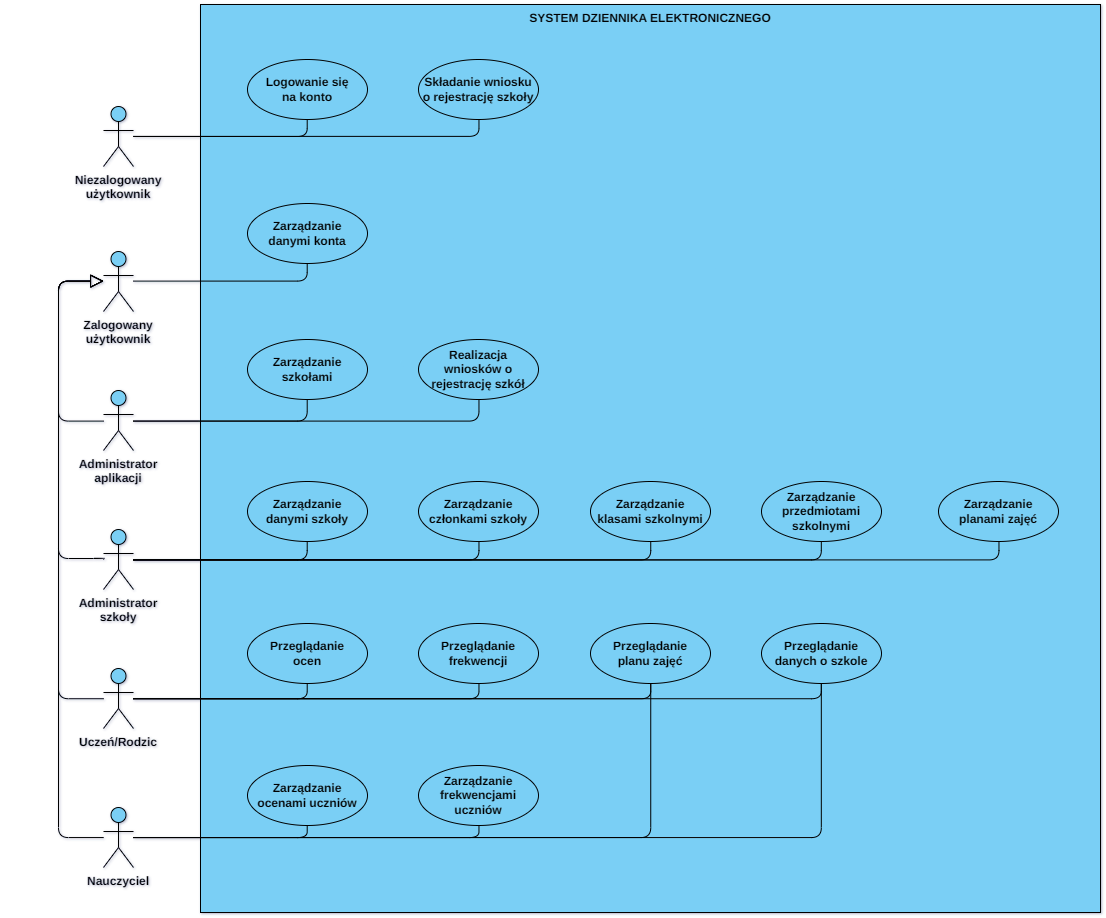
\includegraphics[width=\linewidth]{obrazy/rozdzial_2/diagramy/diagram_przypadkow_uzycia.png}
    \caption{Diagram przypadków użycia systemu dziennika elektronicznego.}
\end{figure}

\newpage

\subsection{Diagramy klas}
Poniższy diagram przedstawia powiązania pomiędzy klasami encji bazodanowych w systemie dziennika elektronicznego.

\begin{figure}[H]
    \centering
    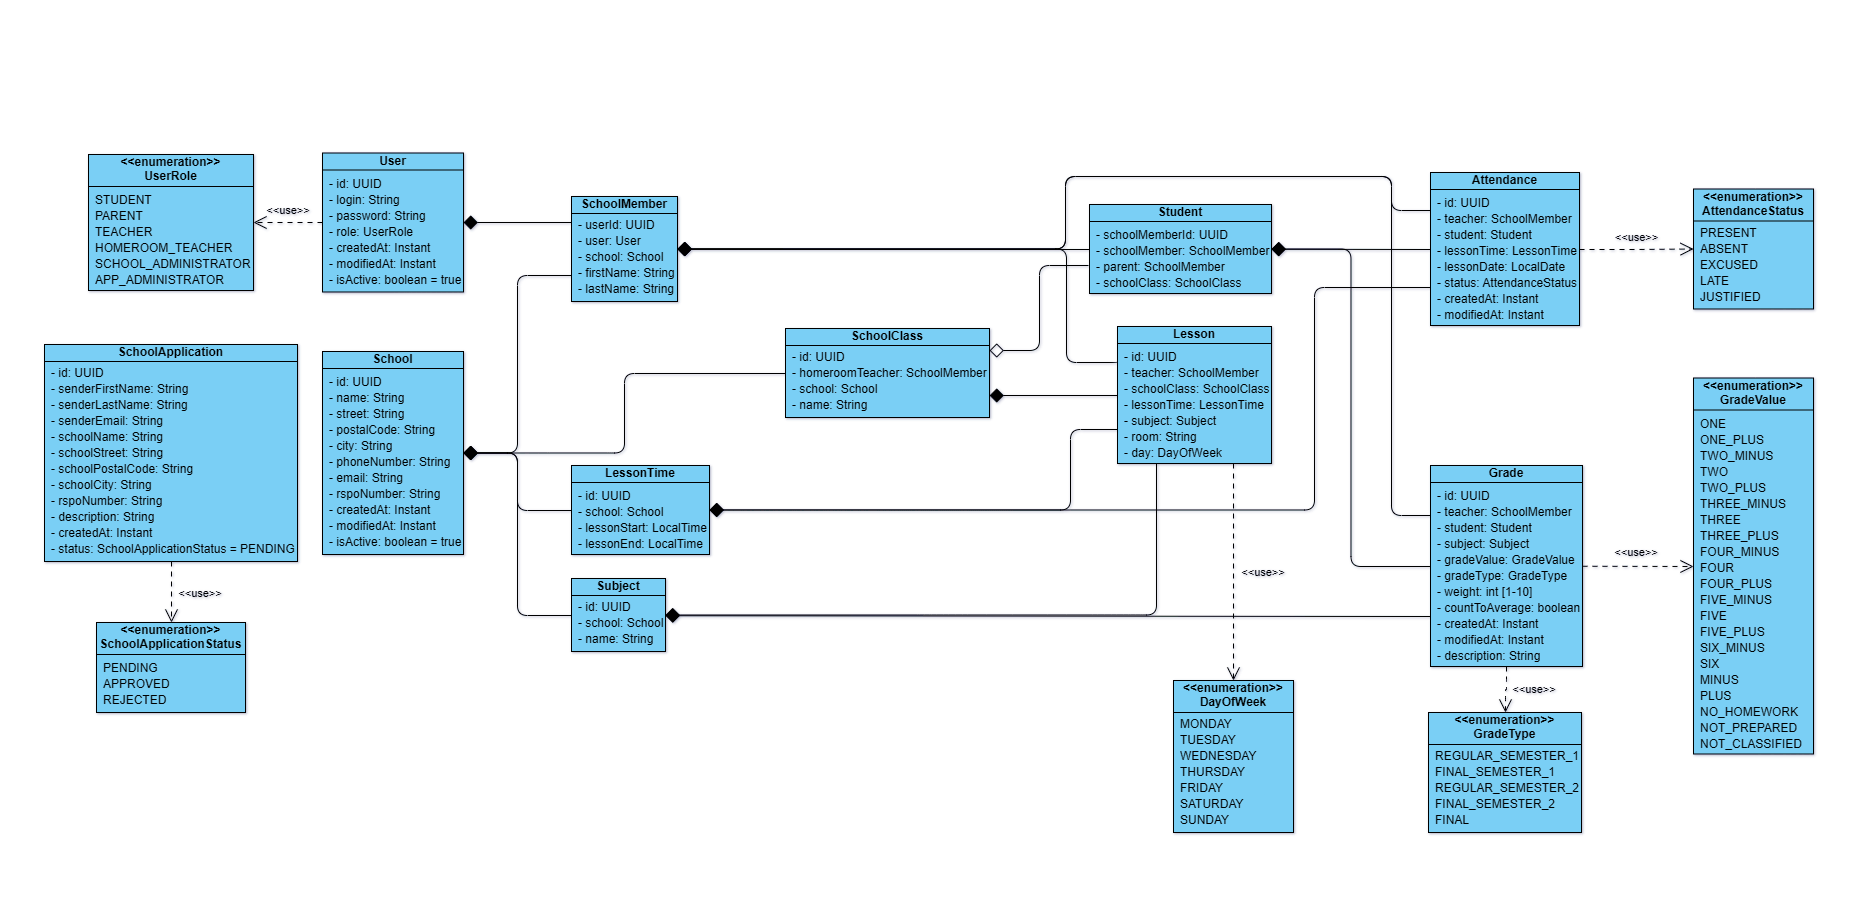
\includegraphics[width=\linewidth]{obrazy/rozdzial_2/diagramy/diagram_klas_encje.png}
    \caption{Struktura klas encji bazodanowych.}
\end{figure}

Aplikacja backedowa zajmująca się logiką biznesową stosuje wyraźny podział klas na:
\begin{itemize}
    \item \textbf{Kontrolery} (\textit{<nazwa\_encji>Controller}) - zajmują się obsługą wystawianego interfejsu REST API.
    \item \textbf{Serwisy} (\textit{<nazwa\_encji>Service}) - zajmują się przetwarzaniem przekazanych danych i realizowaniem logiki biznesowej.
    \item \textbf{Repozytoria} (\textit{<nazwa\_encji>Repository}) - zajmują się komunikacją z bazą danych i wykonywaniem operacji na encjach bazodanowych.
\end{itemize}

Poniższy diagram klas przedstawia powiązania klas dla encji bazodanowej \textbf{User}. Każda inna encja przedstawiona na pierwszym diagramie klas zachowuje podobną strukturę powiązań pomiędzy encjami, repozytoriami, serwisami i kontrolerami.

\begin{figure}[H]
    \centering
    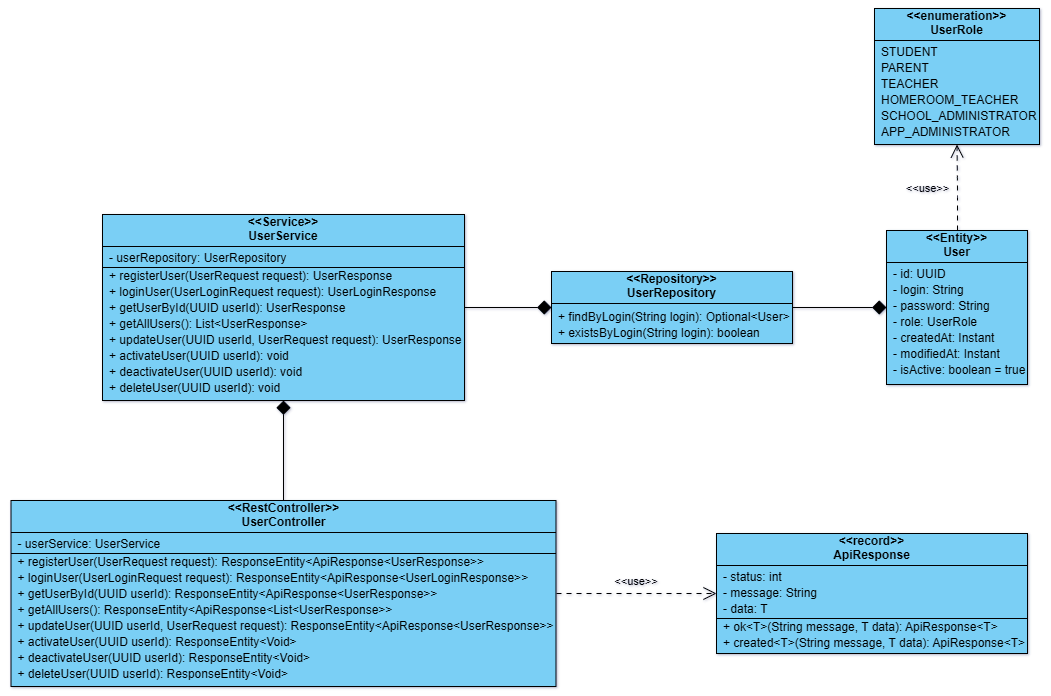
\includegraphics[width=\linewidth]{obrazy/rozdzial_2/diagramy/diagram_klas_uzytkownik.png}
    \caption{Powiązania klas dla encji User.}
\end{figure}

\subsection{Diagram ERD dla relacyjnej bazy danych}
Poniższy diagram przedstawia strukturę danych, która znajduje się bazie danych systemu dziennika elektronicznego.

\begin{figure}[H]
    \centering
    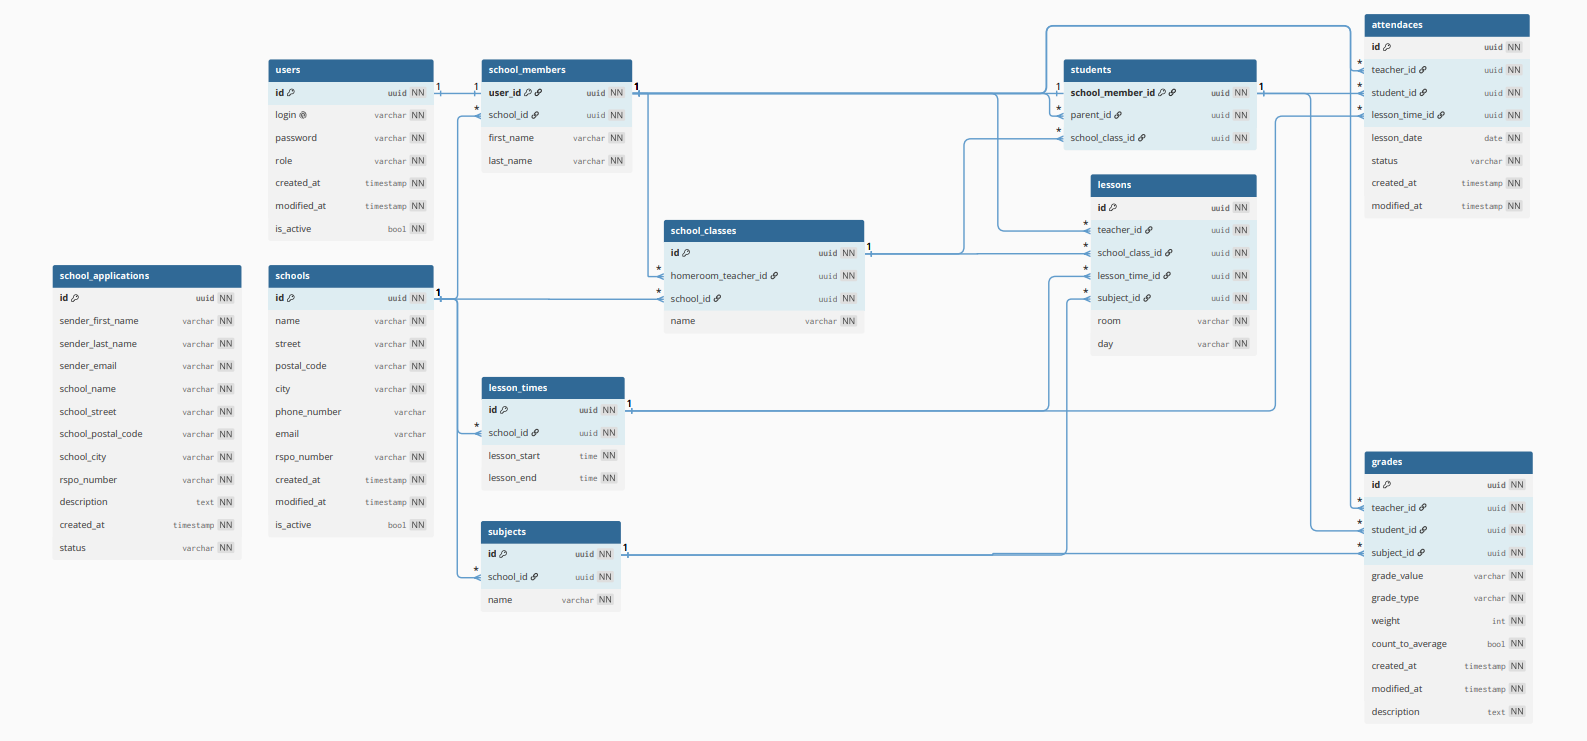
\includegraphics[width=\linewidth]{obrazy/rozdzial_2/diagramy/diagram_zwiazkow_encji.png}
    \caption{Diagram związków encji w bazie danych systemu.}
\end{figure}

\newpage

Wyjaśnienie symboli:
\begin{itemize}
    \item \textbf{NN} (Not Null) - oznacza, że kolumna tabeli nie może mieć pustej wartości (NULL).
    \item \textbf{Klucz} - oznacza, że kolumna tabeli jest kluczem głównym (identyfikatorem).
    \item \textbf{Łańcuch} - oznacza, że kolumna tabeli jest w relacji z inną tabelą.
    \item \textbf{Odcisk palca} - oznacza, że w danej kolumnie tabeli wszystkie wartości są unikalne (występuje tylko przy kolumnie \textbf{\textit{login}} w tabeli \textbf{\textit{users}}).
\end{itemize}

\subsection{Projekt interfejsu użytkownika}
Poniższe grafiki są gotowymi projektami interfejsu użytkownika, które są już zaimplementowane w aplikacji.

\begin{figure}[H]
    \centering
    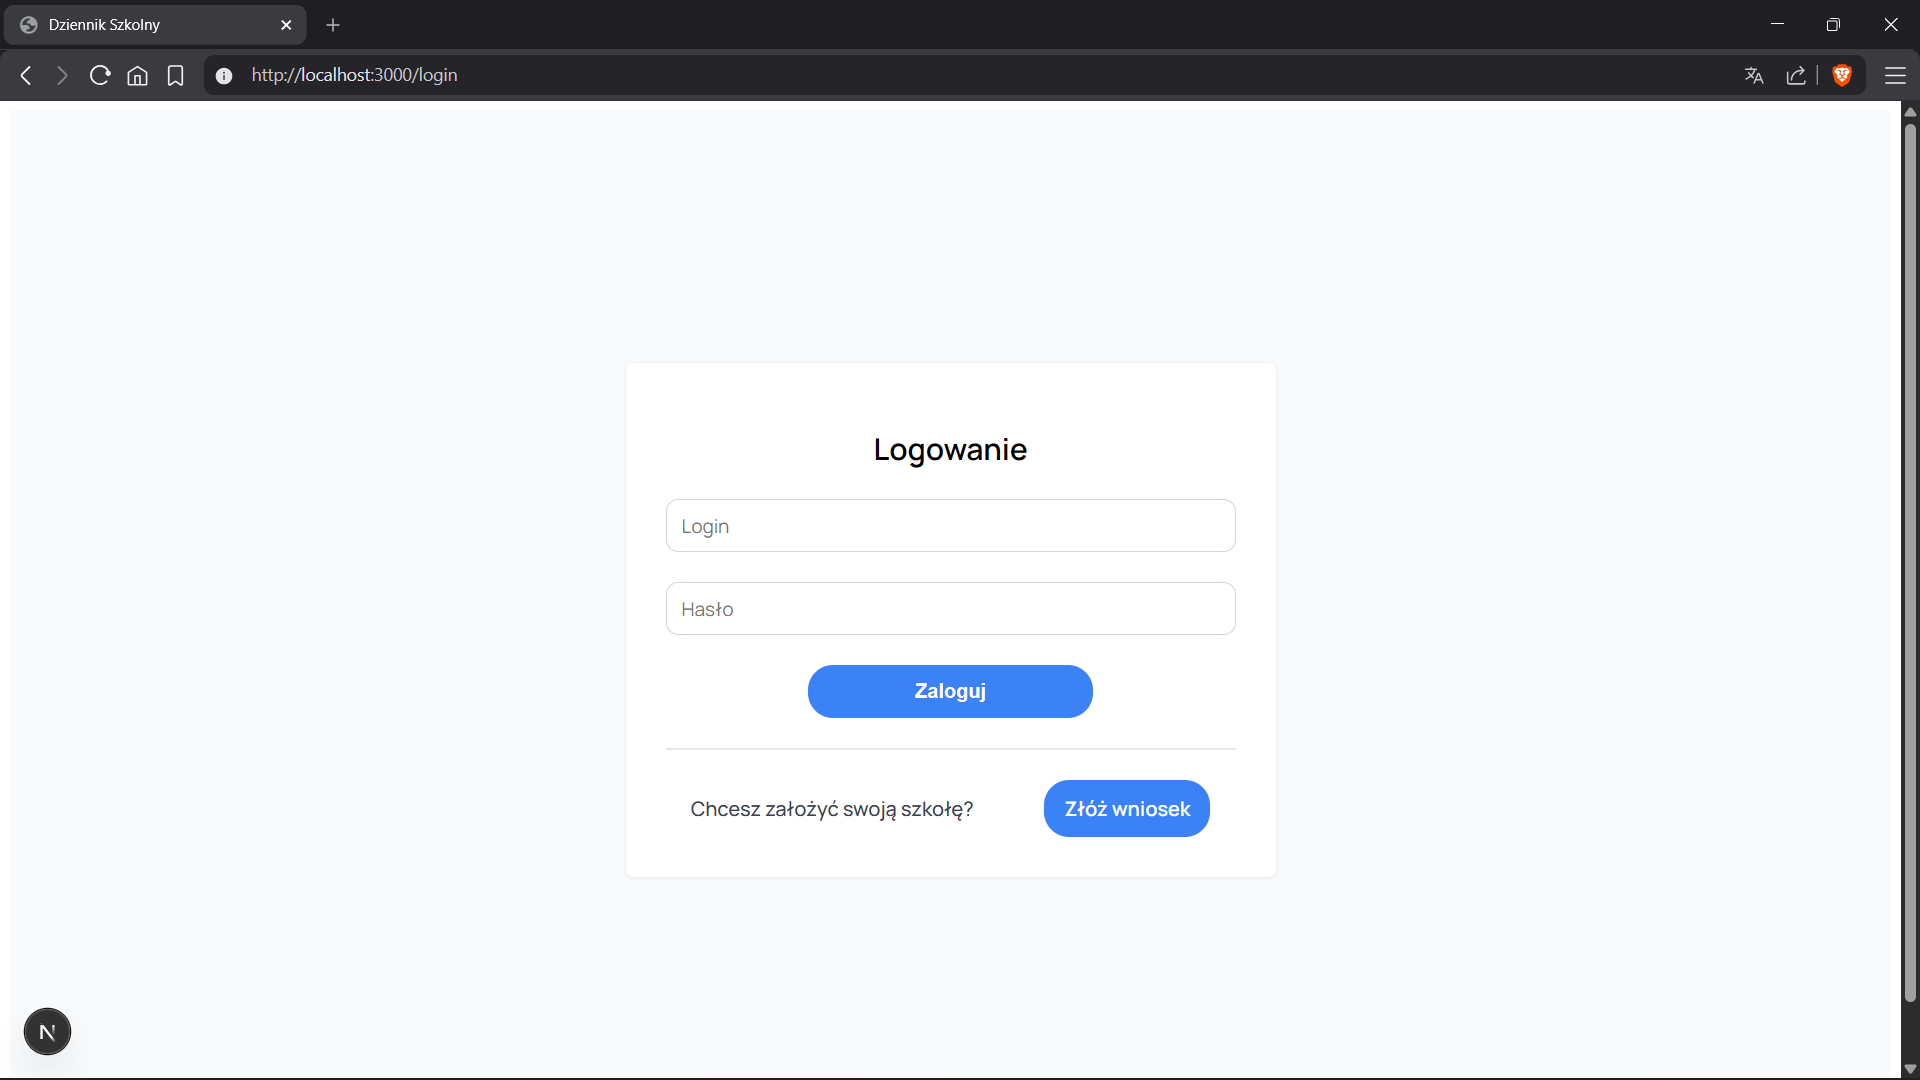
\includegraphics[width=\linewidth]{obrazy/rozdzial_2/interfejs_uzytkownika/logowanie.png}
    \caption{Strona logowania.}
\end{figure}

\begin{figure}[H]
    \centering
    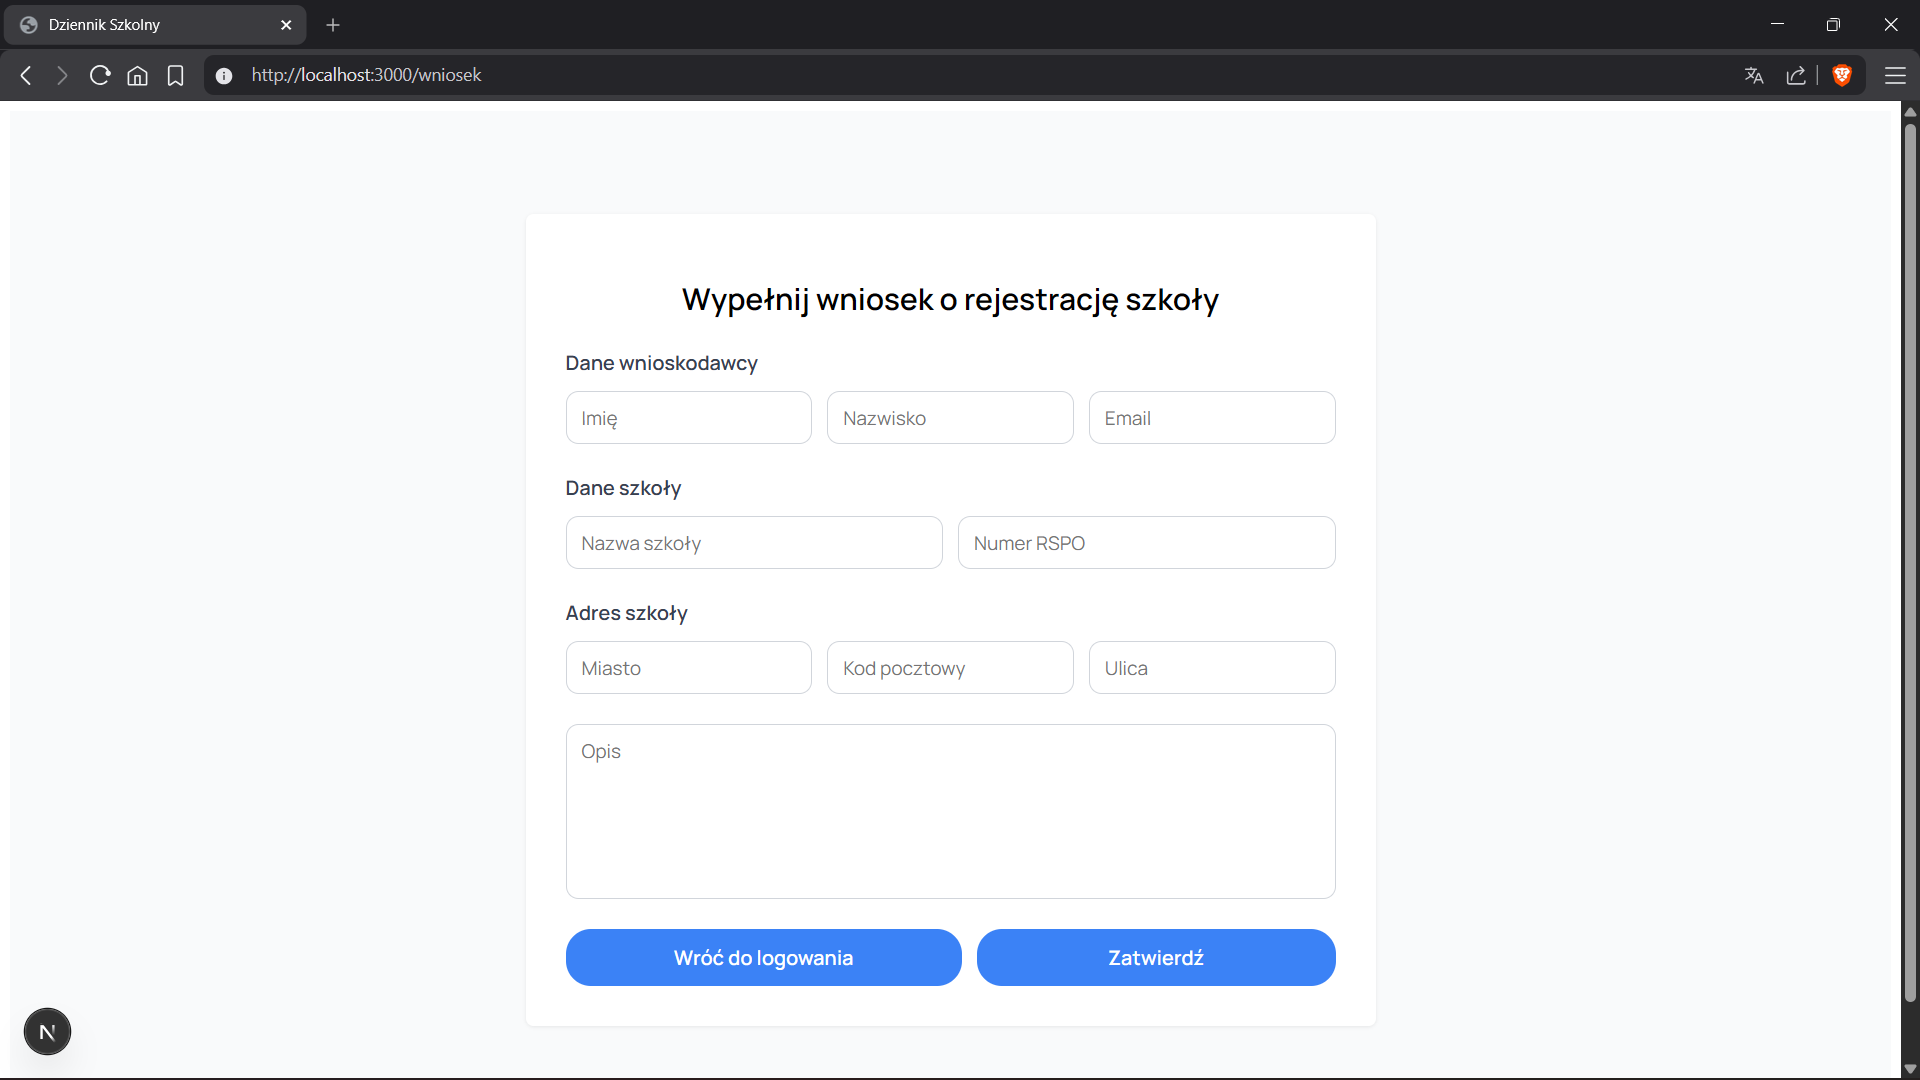
\includegraphics[width=\linewidth]{obrazy/rozdzial_2/interfejs_uzytkownika/wniosek.png}
    \caption{Strona wniosku o rejestrację szkoły w systemie.}
\end{figure}

\begin{figure}[H]
    \centering
    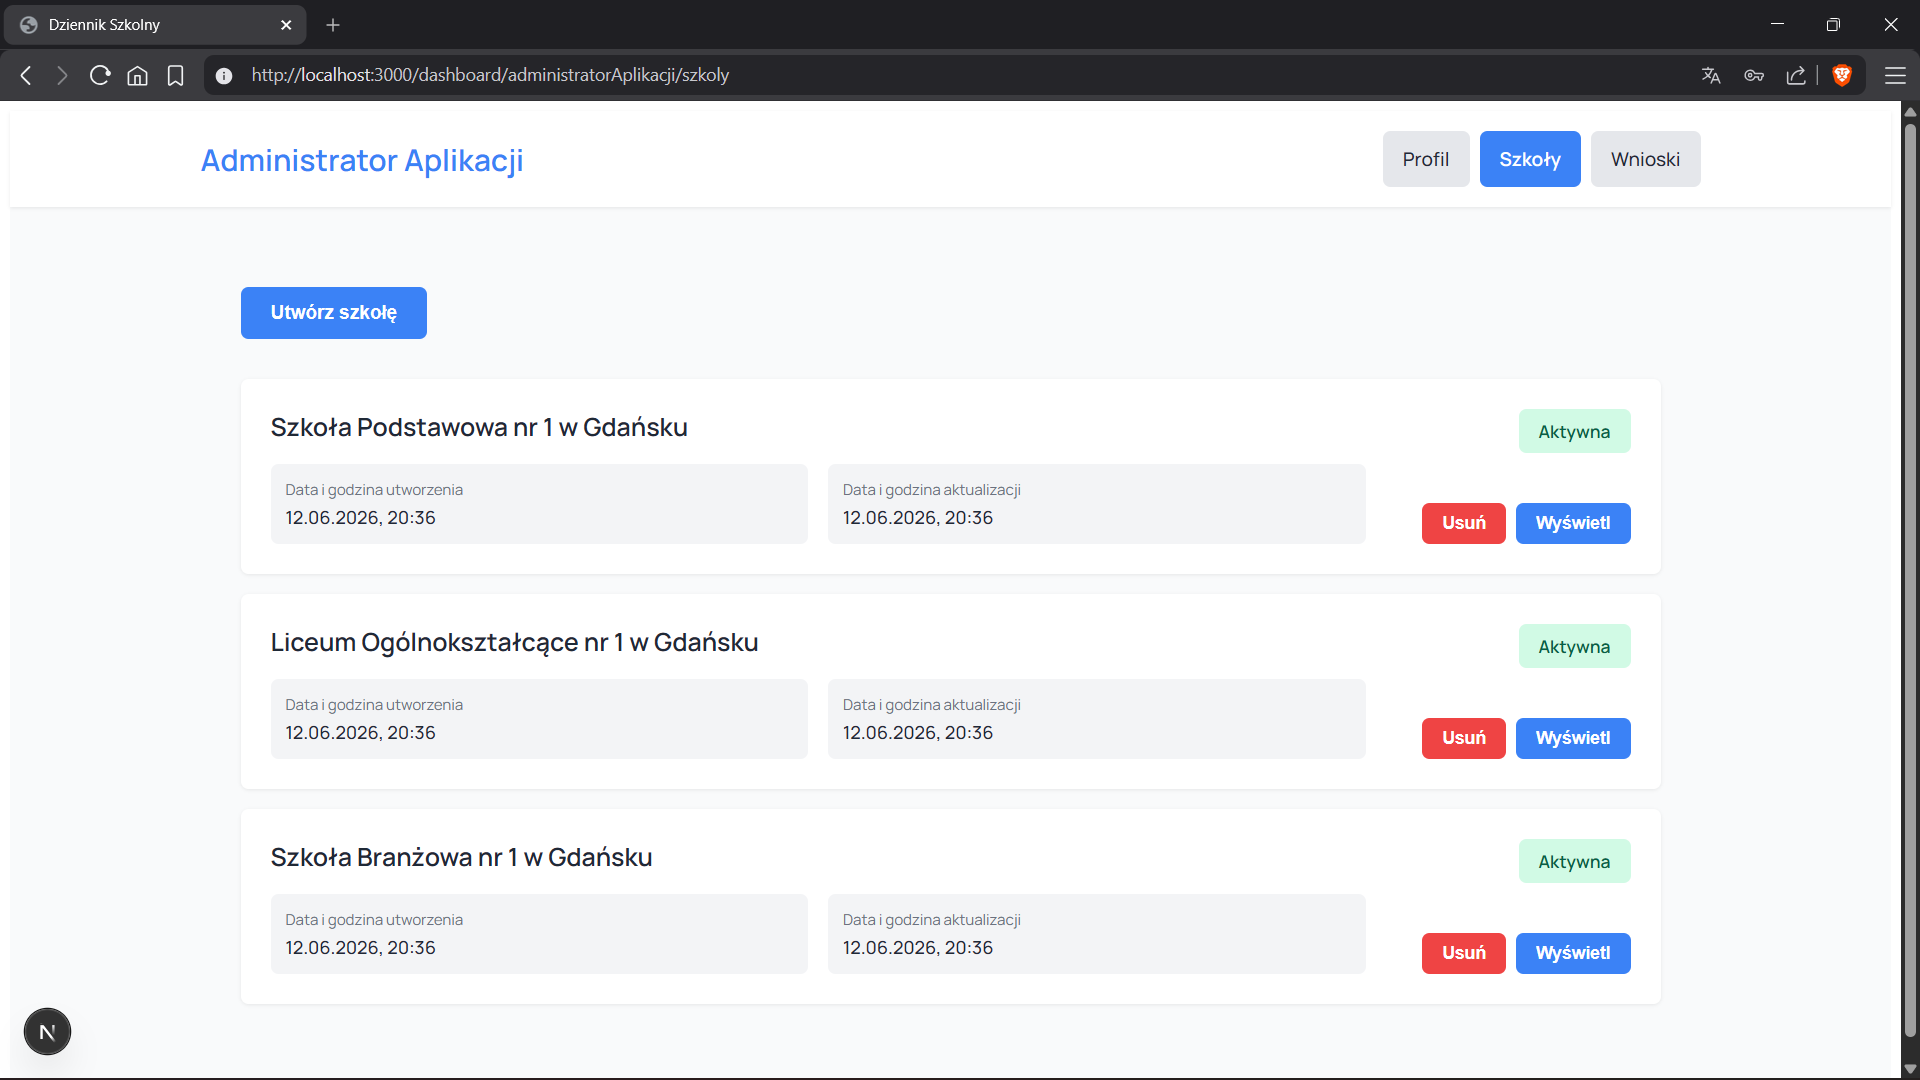
\includegraphics[width=\linewidth]{obrazy/rozdzial_2/interfejs_uzytkownika/panel_administratora_aplikacji.png}
    \caption{Strona panelu administratora aplikacji (lista szkół).}
\end{figure}

\begin{figure}[H]
    \centering
    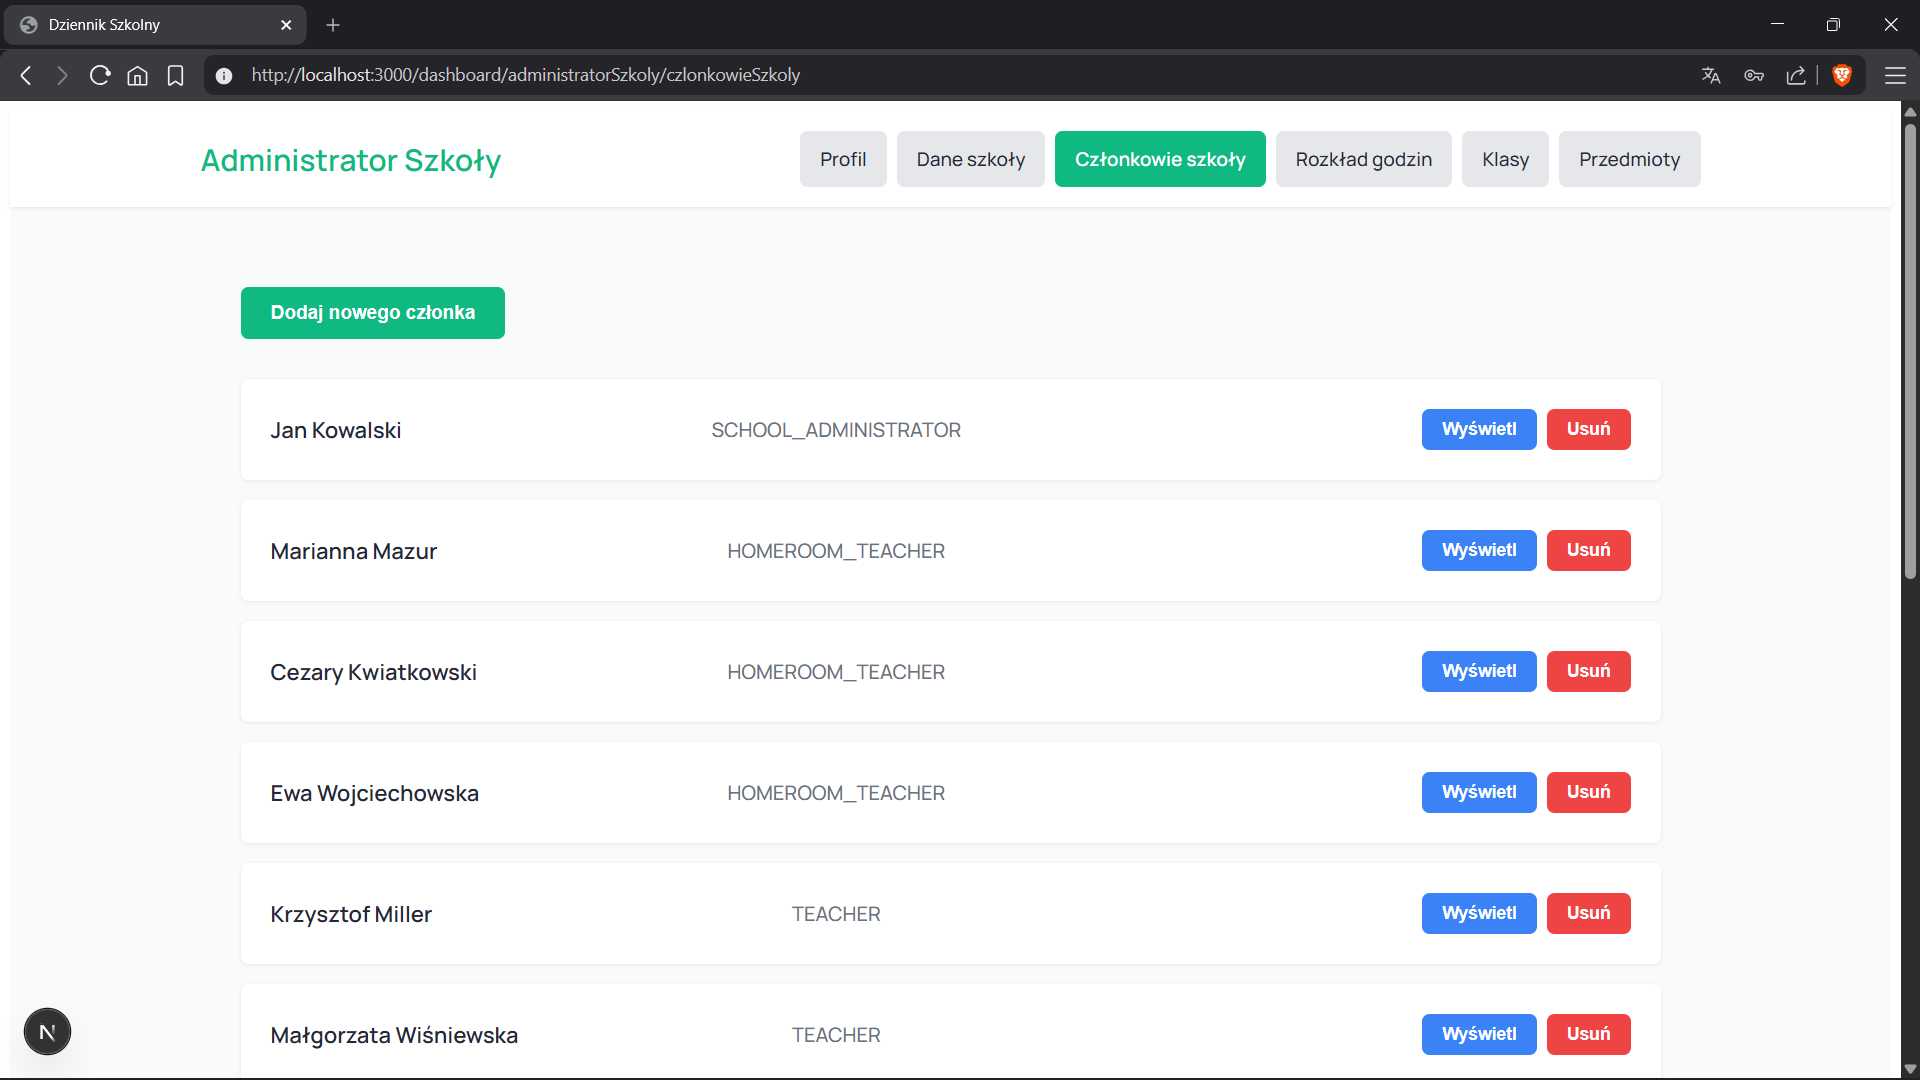
\includegraphics[width=\linewidth]{obrazy/rozdzial_2/interfejs_uzytkownika/panel_administratora_szkoly.png}
    \caption{Strona panelu administratora szkoły (lista członków szkoły).}
\end{figure}

\begin{figure}[H]
    \centering
    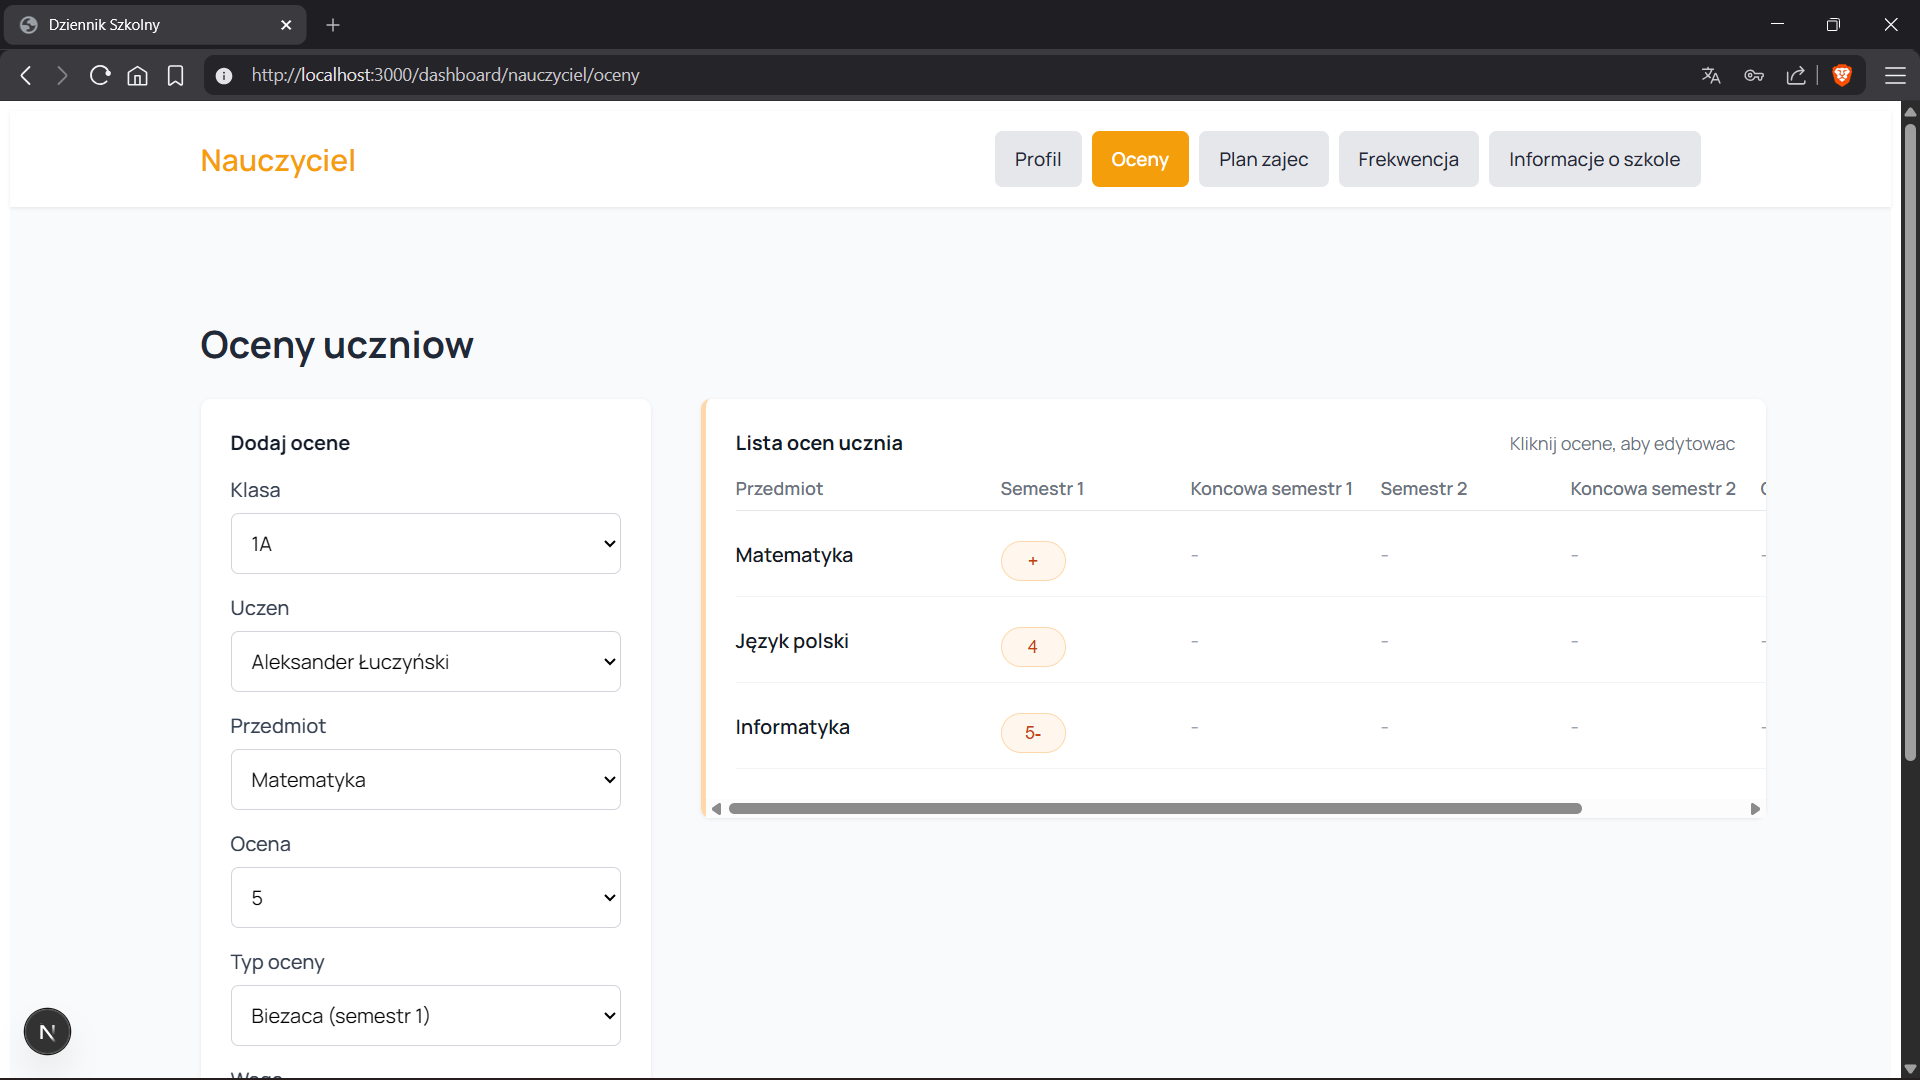
\includegraphics[width=\linewidth]{obrazy/rozdzial_2/interfejs_uzytkownika/panel_nauczyciela.png}
    \caption{Strona panelu nauczyciela (sekcja wystawiania ocen).}
\end{figure}

\begin{figure}
    \centering
    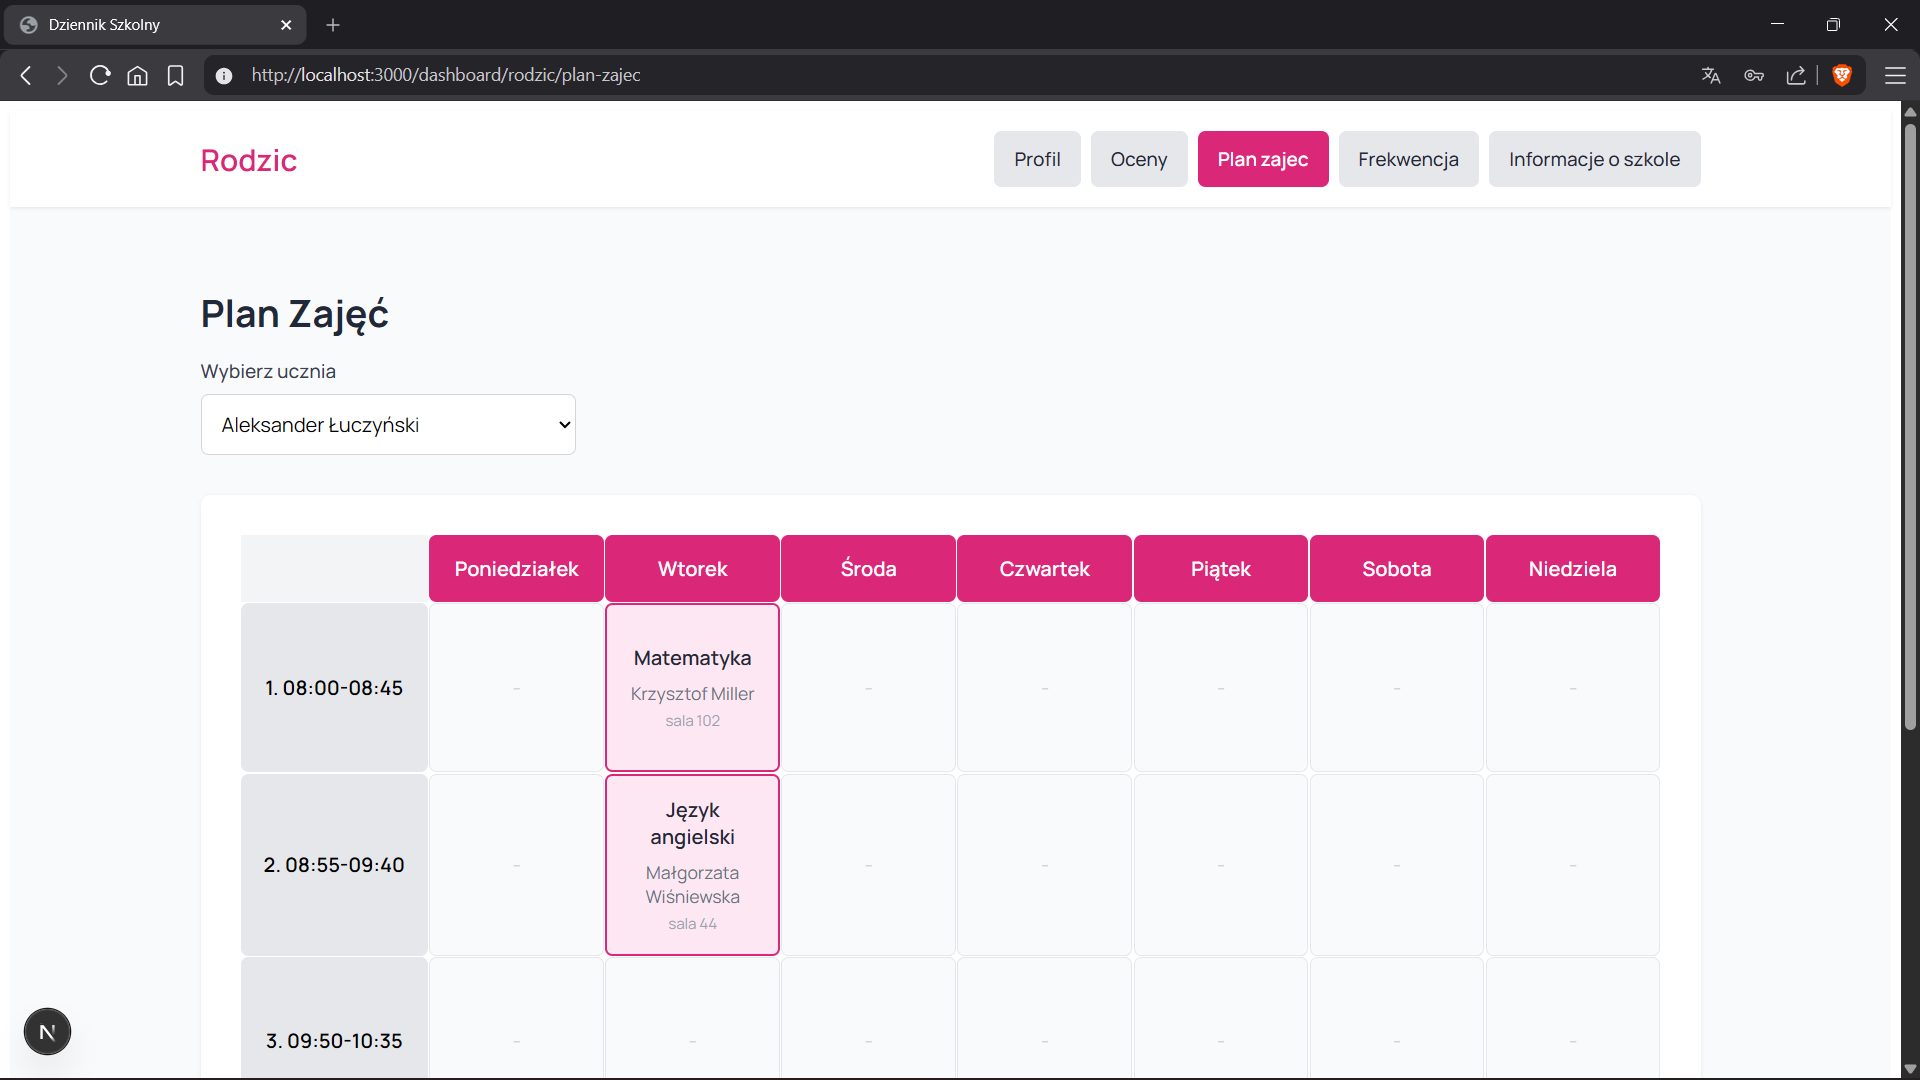
\includegraphics[width=\linewidth]{obrazy/rozdzial_2/interfejs_uzytkownika/panel_rodzica.png}
    \caption{Strona panelu rodzica (plan lekcji wybranego ucznia).}
\end{figure}

\begin{figure}[H]
    \centering
    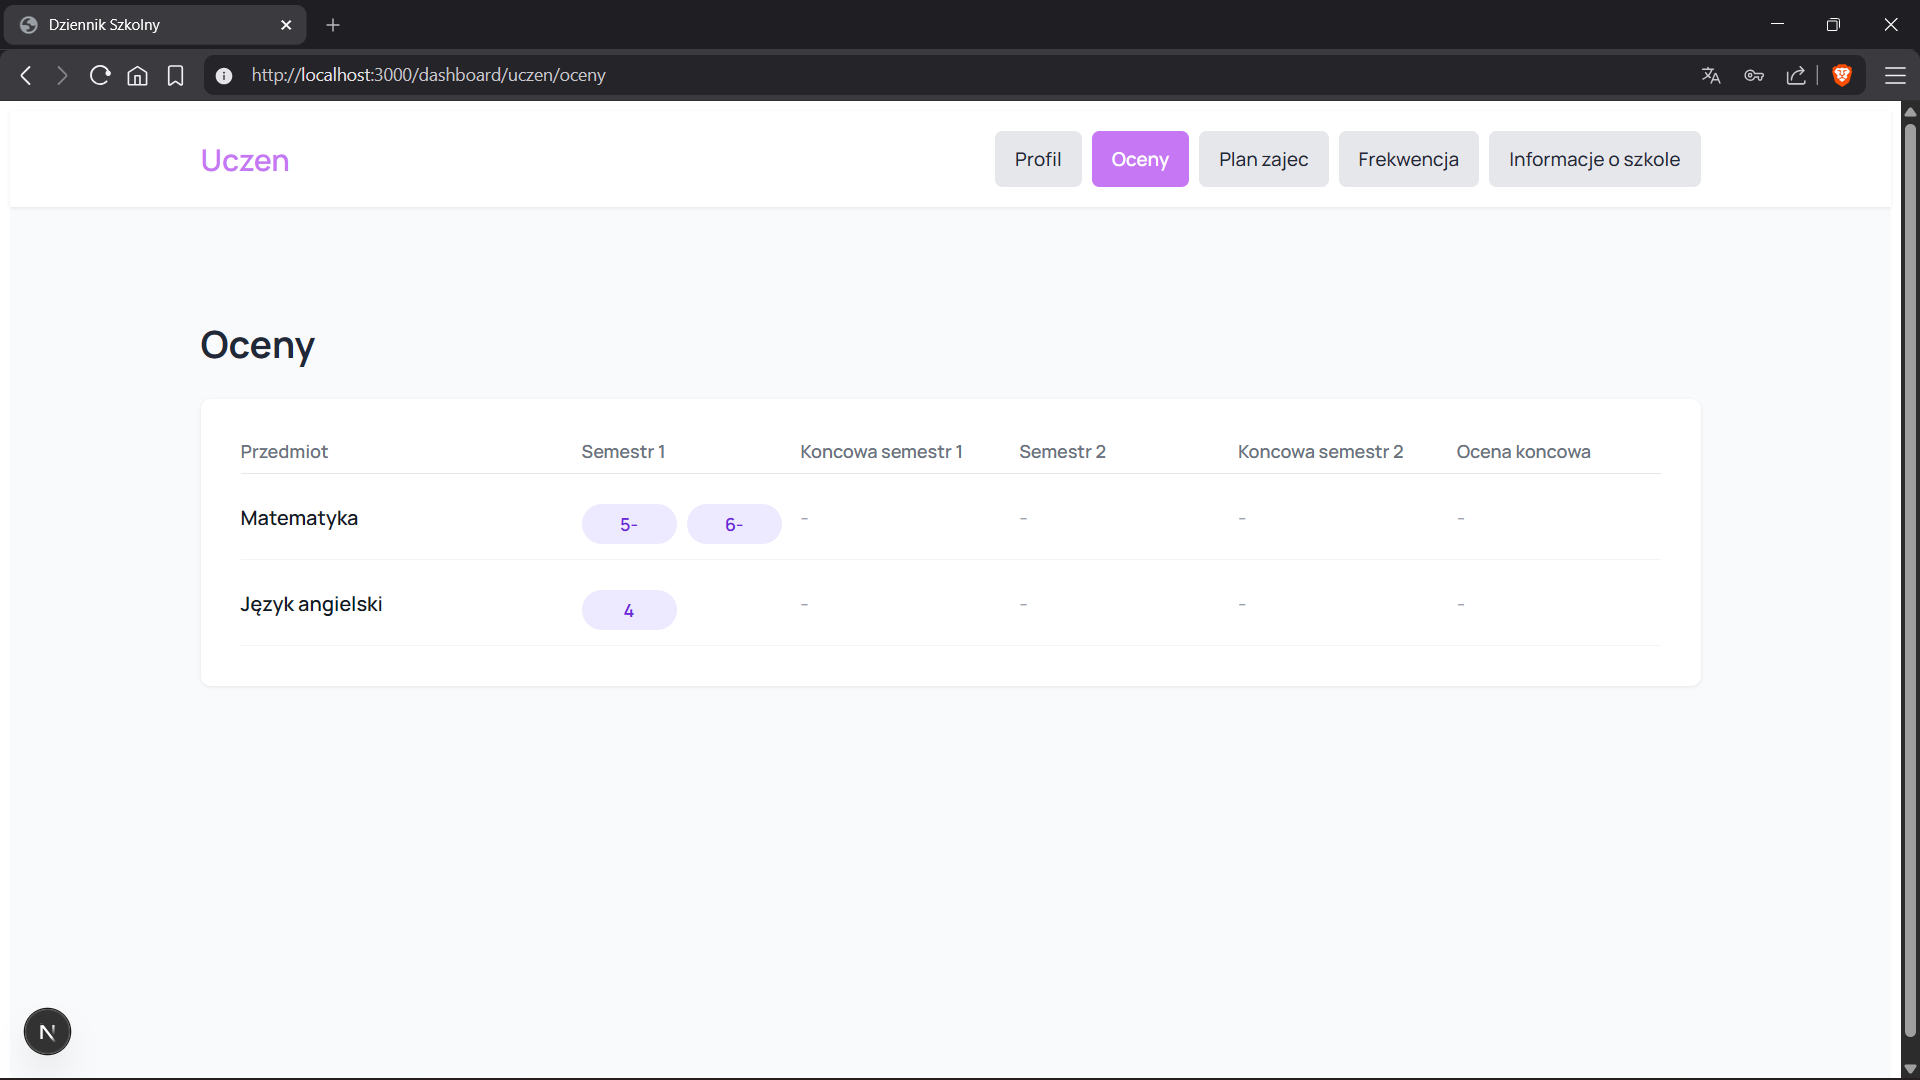
\includegraphics[width=\linewidth]{obrazy/rozdzial_2/interfejs_uzytkownika/panel_ucznia.png}
    \caption{Strona panelu ucznia (lista ocen).}
\end{figure}

% ========================= ROZDZIAŁ 3 =========================
\section{Implementacja}
\subsection{Architektura całości systemu}
System dziennika elektronicznego został wykonany w architekturze monolitycznej i zawiera 3 główne komponenty:

\begin{itemize}
    \item Aplikacja frontendowa
    \item Aplikacja backendowa
    \item Baza danych
\end{itemize}

Poniższy diagram przedstawia główną architekturę systemu.

\begin{figure}[H]
    \centering
    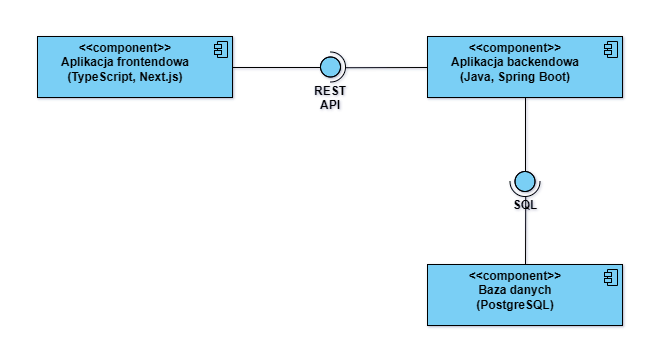
\includegraphics[width=\linewidth]{obrazy/rozdzial_3/diagramy/diagram_komponentow.png}
    \caption{Diagram architektury systemu dziennika elektronicznego.}
\end{figure}

\subsection{Użyte wzorce projektowe}
System dziennika elektronicznego realizuje poniższe wzorce projektowe:
\begin{itemize}
    \item \textbf{REST} (\textit{Representational State Transfer}) - aplikacje frontendowa i backendowa komunikują się przez protokół HTTP oraz interfejs REST API wystawiany przez backend. Dane są wymieniane w formacie JSON. Dzięki temu wzorcowi, dane są w prosty sposób przesyłane pomiędzy aplikacjami.
    \item \textbf{ORM} (\textit{Object-Relational Mapping}) - aplikacja backendowa używa mapowania obiektowo-relacyjnego, aby komunikować się z bazą danych. Dzięki temu wzorcowi, zapytania do bazy danych można formułować przy pomocy obiektów klas, a nie używając języka SQL.
\end{itemize}

\subsection{Diagramy sekwencji przedstawiające funkcjonalności systemu}
\begin{figure}[H]
    \centering
    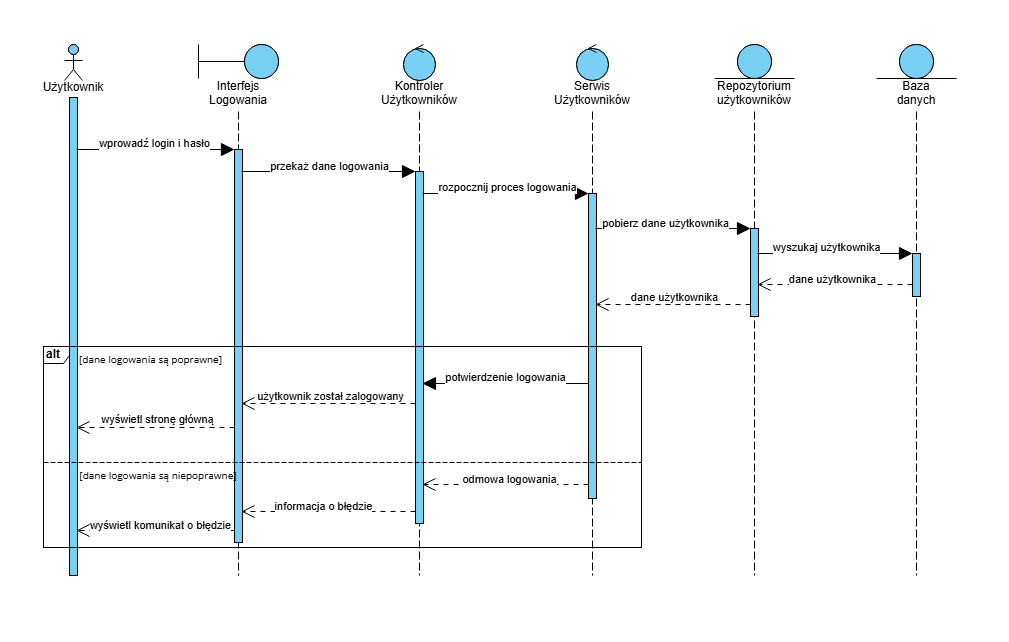
\includegraphics[width=\linewidth]{obrazy/rozdzial_3/diagramy/diagram_sekwencji_logowanie.png}
    \caption{Logowanie do systemu}
\end{figure}

Powyższy diagram przedstawia logowanie się użytkownika do systemu dziennika elektronicznego. \textbf{\textit{Użytkownik}} wprowadza dane logowania w \textbf{\textit{Interfejsie logowania}}, które są przekazywane do warstwy \textbf{\textit{Kontrolera użytkowników}} i \textbf{\textit{Serwisu użytkowników}} odpowiedzialnego za obsługę logowania. Serwis pobiera dane użytkownika z \textbf{\textit{Repozytorium użytkowników}}, które komunikuje się z \textbf{\textit{Bazą danych}} w celu odnalezienia odpowiedniego konta. Po weryfikacji poprawności danych logowania system zwraca informację o pomyślnym logowaniu i wyświetla użytkownikowi stronę główną aplikacji. W przypadku podania niepoprawnych danych użytkownik otrzymuje komunikat o błędzie i nie ma dostępu do systemu.

\begin{figure}[H]
    \centering
    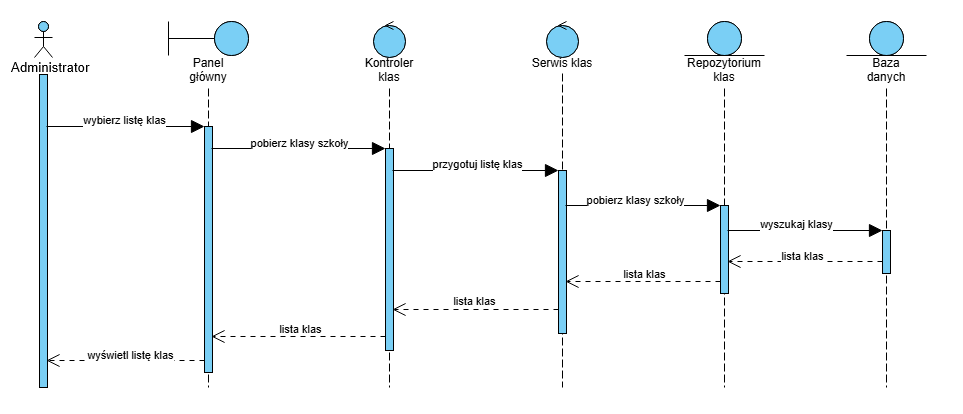
\includegraphics[width=\linewidth]{obrazy/rozdzial_3/diagramy/diagram_sekwencji_wyswietlanie_klas.png}
    \caption{Wyświetlanie listy klas}
\end{figure}

Powyższy diagram obrazuje proces pobierania i wyświetlania listy klas przypisanych do szkoły. \textbf{\textit{Administrator}} wykonuje operację poprzez swój \textbf{\textit{Panel główny}}. Jego żądanie jest przekierowane do \textbf{\textit{Kontrolera klas}}, który następnie deleguje pobranie danych do \textbf{\textit{Serwisu klas}}. Serwis komunikuje się z \textbf{\textit{Repozytorium klas}} odpowiedzialnym za dostęp do danych zapisanych w \textbf{\textit{Bazie danych}}. Po pobraniu listy klas informacje są zwracane do interfejsu użytkownika, gdzie są one wyświetlane w formie listy.

\begin{figure}[H]
    \centering
    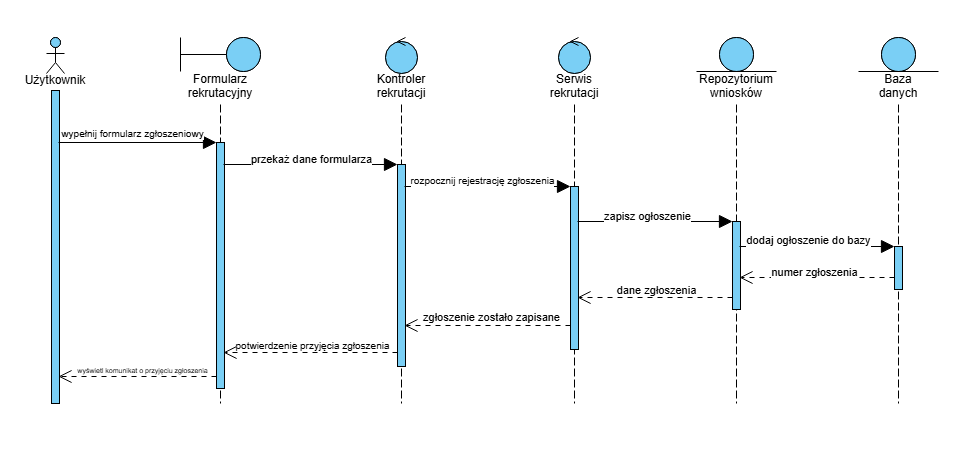
\includegraphics[width=\linewidth]{obrazy/rozdzial_3/diagramy/diagram_sekwencji_zgloszenia.png}
    \caption{Składanie wniosku o utworzenie szkoły}
\end{figure}

Powyższy diagram przedstawia proces składania wniosku o utworzenie szkoły przez \textbf{\textit{Użytkownika}}. Wypełnia on \textbf{\textit{Formularz rekrutacyjny}} i przesyła go do systemu. Tam dane formularza są przekazywane przez \textbf{\textit{Kontroler rekrutacji}} do \textbf{\textit{Serwisu rekrutacji}}, który obsługuje proces rejestracji zgłoszeń. Serwis zapisuje zgłoszenia przy użyciu \textbf{\textit{Repozytorium wniosków}}, które komunikuje się z \textbf{\textit{Bazą danych}}. Po poprawnym zapisaniu zgłoszenia system generuje numer identyfikacyjny zgłoszenia i zwraca użytkownikowi potwierdzenie przyjęcia jego wniosku.

\begin{figure}[H]
    \centering
    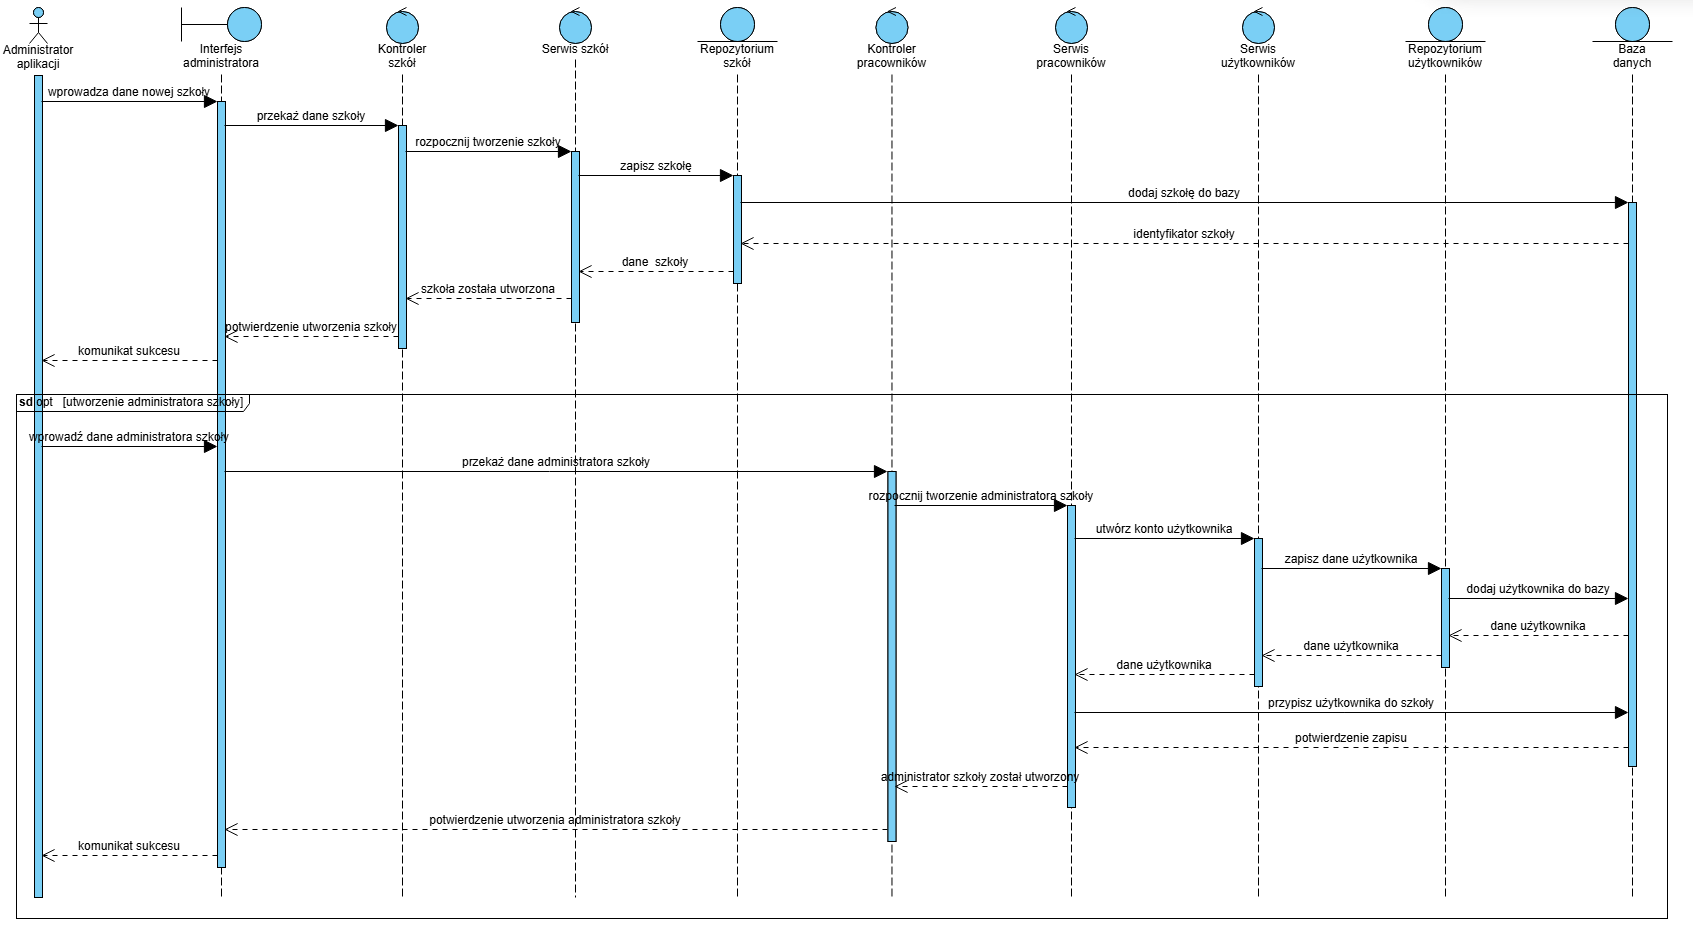
\includegraphics[width=\linewidth]{obrazy/rozdzial_3/diagramy/diagram_sekwencji_tworzenie_szkoly_i_admina.png}
    \caption{Utworzenie szkoły i przypisanie jej administratora}
\end{figure}

Powyższy diagram pokazuje sposób w jaki \textbf{\textit{Administrator aplikacji}} dodaje nową szkołę do systemu oraz opcjonalnie przypisuje do niej administratora szkoły. Najpierw przy pomocy swojego \textbf{\textit{Interfejsu}} wprowadza dane nowej placówki, które następnie są przekazywane do \textbf{\textit{Kontrolera szkół}} i dalej do \textbf{\textit{Serwisu szkół}}, który jest odpowiedzialny za zarządzanie szkołami. Następnie dane są zapisywane w \textbf{\textit{Bazie danych}} za pośrednictwem \textbf{\textit{Repozytorium szkół}}. Po pomyślnym utworzeniu szkoły administrator aplikacji otrzymuje komunikat o tym, że udało mu się zakończyć proces oraz otrzymuje on możliwość dodania do niej administratora szkoły. Dane nowego użytkownika są przekazywane do \textbf{\textit{Kontrolera pracowników}}. Następnie poprzez \textbf{\textit{Serwis pracowników}} i \textbf{\textit{Serwis użytkowników}}, dane użytkownika zostają zapisane w bazie danych przez \textbf{\textit{Repozytorium użytkowników}}. Po utworzeniu konta dla administratora zostaje on przypisany do wcześniej stworzonej szkoły. Po zakończeniu procesu system wyświetla administratorowi aplikacji komunikat o prawidłowym wykonaniu operacji.

\begin{figure}[H]
    \centering
    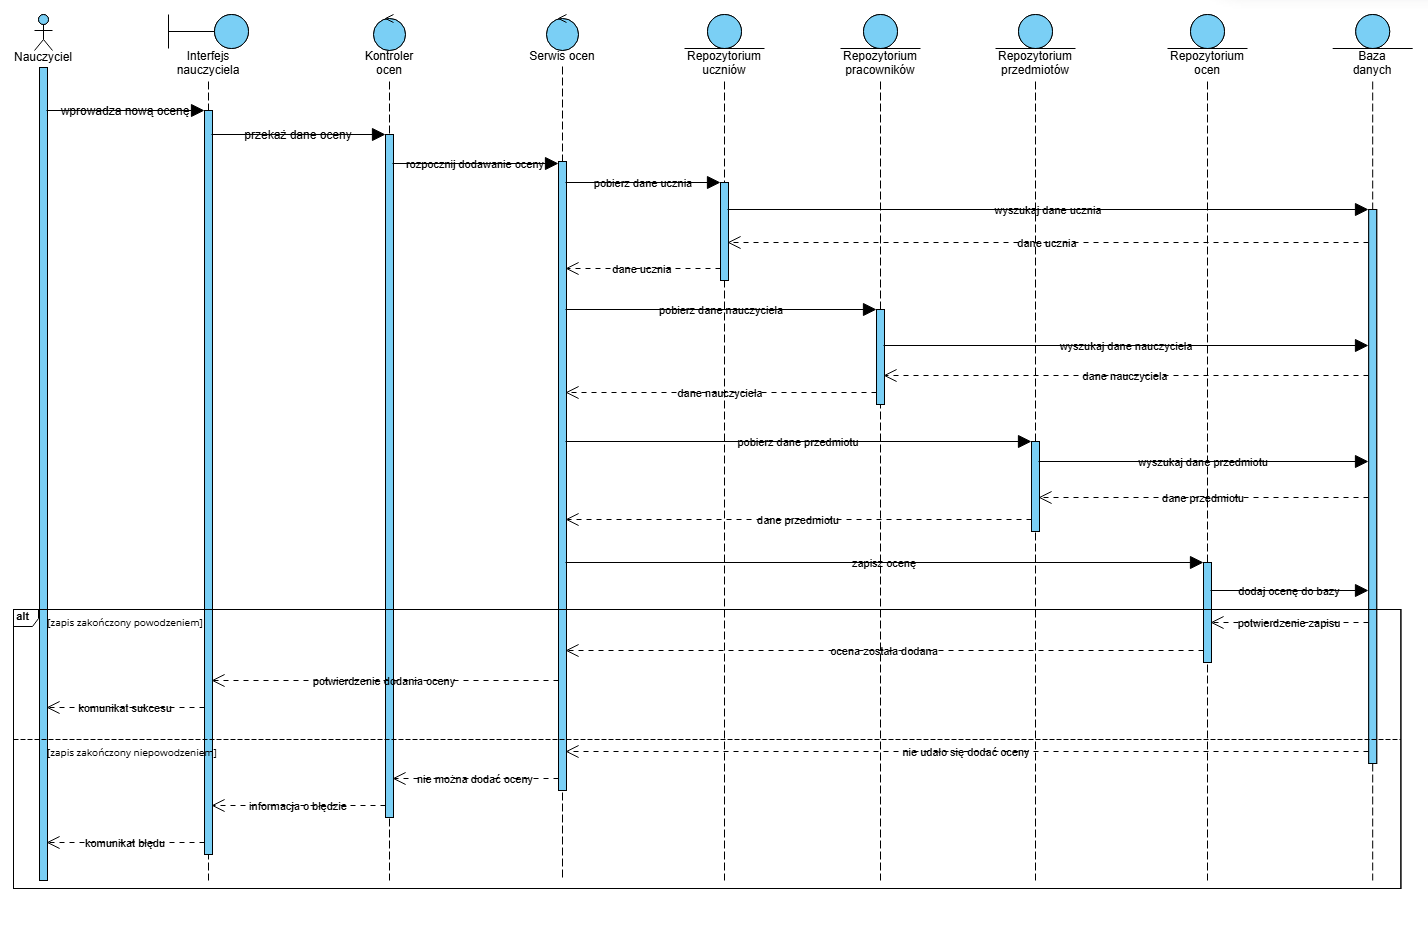
\includegraphics[width=\linewidth]{obrazy/rozdzial_3/diagramy/diagram_sekwencji_wprowadzanie_oceny.png}
    \caption{Wpisywanie oceny}
\end{figure}

Powyższy diagram przedstawia proces wystawiania oceny przez \textbf{\textit{Nauczyciela}}. Nauczyciel wprowadza dane oceny w \textbf{\textit{Interfejsie nauczyciela}}, skąd zostają one przekazane do \textbf{\textit{Kontrolera ocen}} oraz \textbf{\textit{Serwisu ocen}}. W celu poprawnego utworzenia wpisu serwis pobiera informacje o: uczniu z \textbf{\textit{Repozytorium uczniów}}, nauczycielu z \textbf{\textit{Repozytorium pracowników}} i przedmiocie z \textbf{\textit{Repozytorium przedmiotów}}. Po otrzymaniu wszystkich wymaganych danych serwis zapisuje ocenę poprzez \textbf{\textit{Repozytorium ocen}}, które komunikuje się z \textbf{\textit{Bazą danych}}. W przypadku poprawnego wykonania operacji nauczyciel otrzymuje potwierdzenie dodania oceny. Jeżeli podczas zapisu wystąpi jakiś błąd, system zwraca odpowiedni komunikat informujący o niepowodzeniu operacji.

\subsection{Użyte technologie w projekcie systemu}
\paragraph{Aplikacja frontendowa}
\begin{itemize}
    \item Użyty język programowania: TypeScript
    \item Użyty framework: Next.js
    \item Użyte biblioteki produkcyjne: React, React DOM, Next
    \item Użyte biblioteki deweloperskie: Tailwind CSS, ESlint, React Testing Library, Vitest
\end{itemize}

\paragraph{Aplikacja backendowa}
\begin{itemize}
    \item Użyty język programowania: Java
    \item Użyty framework: Spring Boot
    \item Użyte biblioteki produkcyjne: Spring Data JPA, Spring Web, PostgreSQL Driver
    \item Użyte biblioteki deweloperskie: Spring Data JPA Test, Spring Web Test, JUnit, JaCoCo, Lombok
\end{itemize}

% ========================= ROZDZIAŁ 4 =========================
\section{Testy}
\subsection{Analiza testów części frontendowej aplikacji}
\subsubsection{Zakres testów}
Testy frontendu aplikacji obejmowały weryfikację funkcjonalności poprzez:
\begin{itemize}
    \item 39 testów jednostkowych (Vitest).
    \item 124 testy komponentów (Vitest + React Testing Library).
    \item Pokrycie kodu na poziomie ok. 83\% (według v8 coverage).
\end{itemize}

Do pokrycia kodu wykorzystano narzędzie v8 coverage, które dostarcza szczegółowych informacji na temat wykonanych linii kodu, gałęzi warunkowych, metod i funkcji podczas testów automatycznych.

\begin{figure}[H]
    \centering
    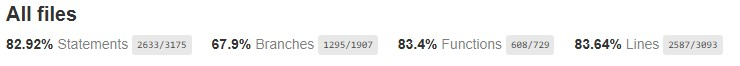
\includegraphics[width=1\textwidth]{obrazy/rozdzial_4/frontend/pokrycie_kodu_ogolne.jpg}
    \caption{Ogólne statystyki pokrycia kodu według v8 coverage}
\end{figure}

\begin{figure}[H]
    \centering
    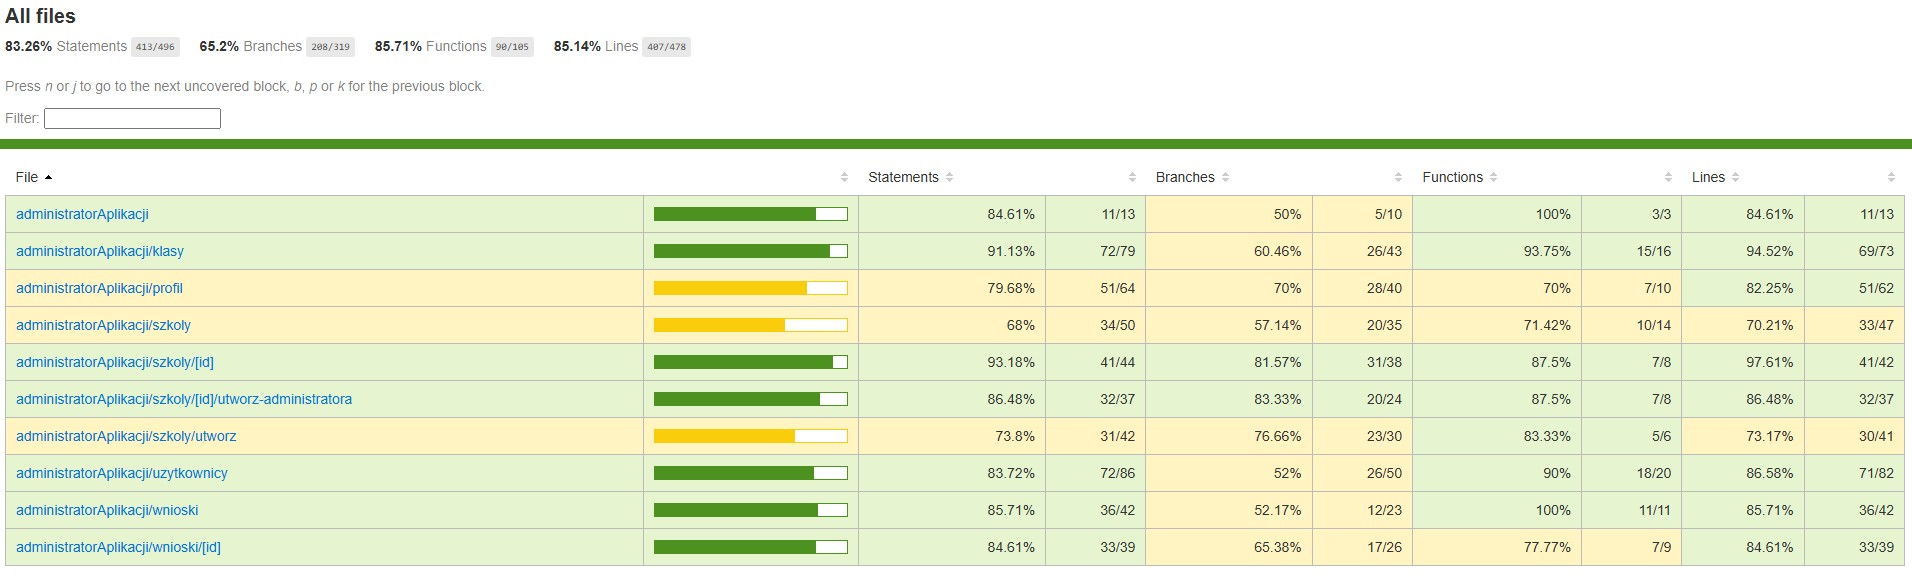
\includegraphics[width=1\textwidth]{obrazy/rozdzial_4/frontend/pokrycie_kodu_admin_aplikacji.jpg}
    \caption{Pokrycie kodu dla modułu administratorAplikacji}
\end{figure}

\begin{figure}[H]
    \centering
    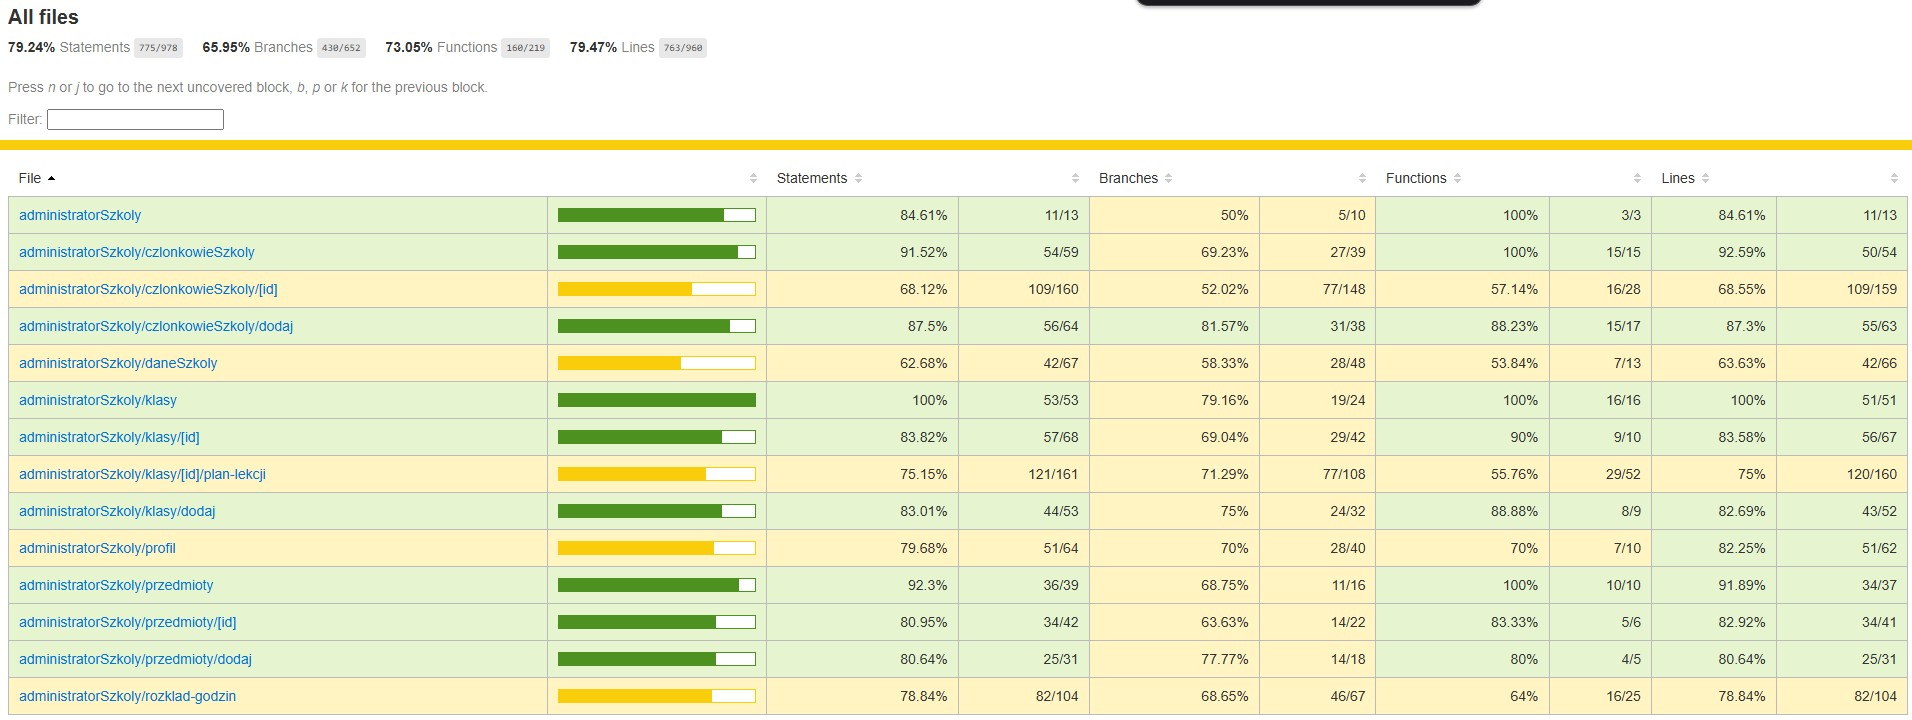
\includegraphics[width=1\textwidth]{obrazy/rozdzial_4/frontend/pokrycie_kodu_admin_szkoly.jpg}
    \caption{Pokrycie kodu dla modułu administratorSzkoly}
\end{figure}

\begin{figure}[H]
    \centering
    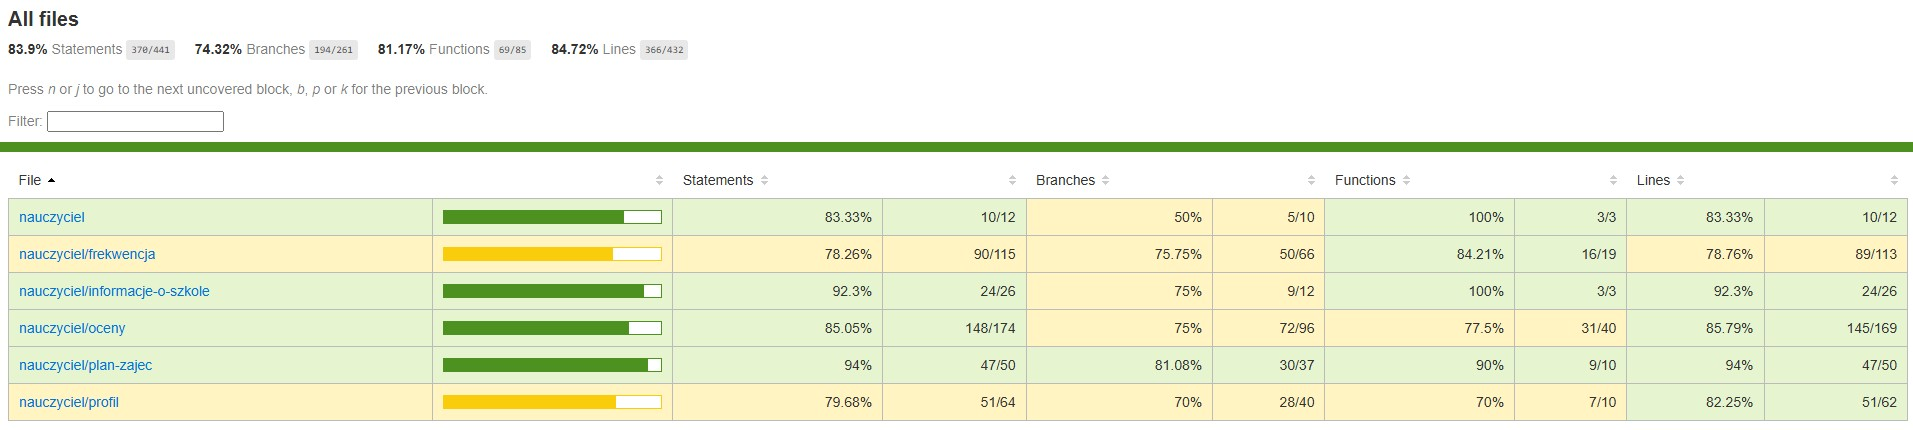
\includegraphics[width=1\textwidth]{obrazy/rozdzial_4/frontend/pokrycie_kodu_nauczyciel.jpg}
    \caption{Pokrycie kodu dla modułu nauczyciel}
\end{figure}

\begin{figure}[H]
    \centering
    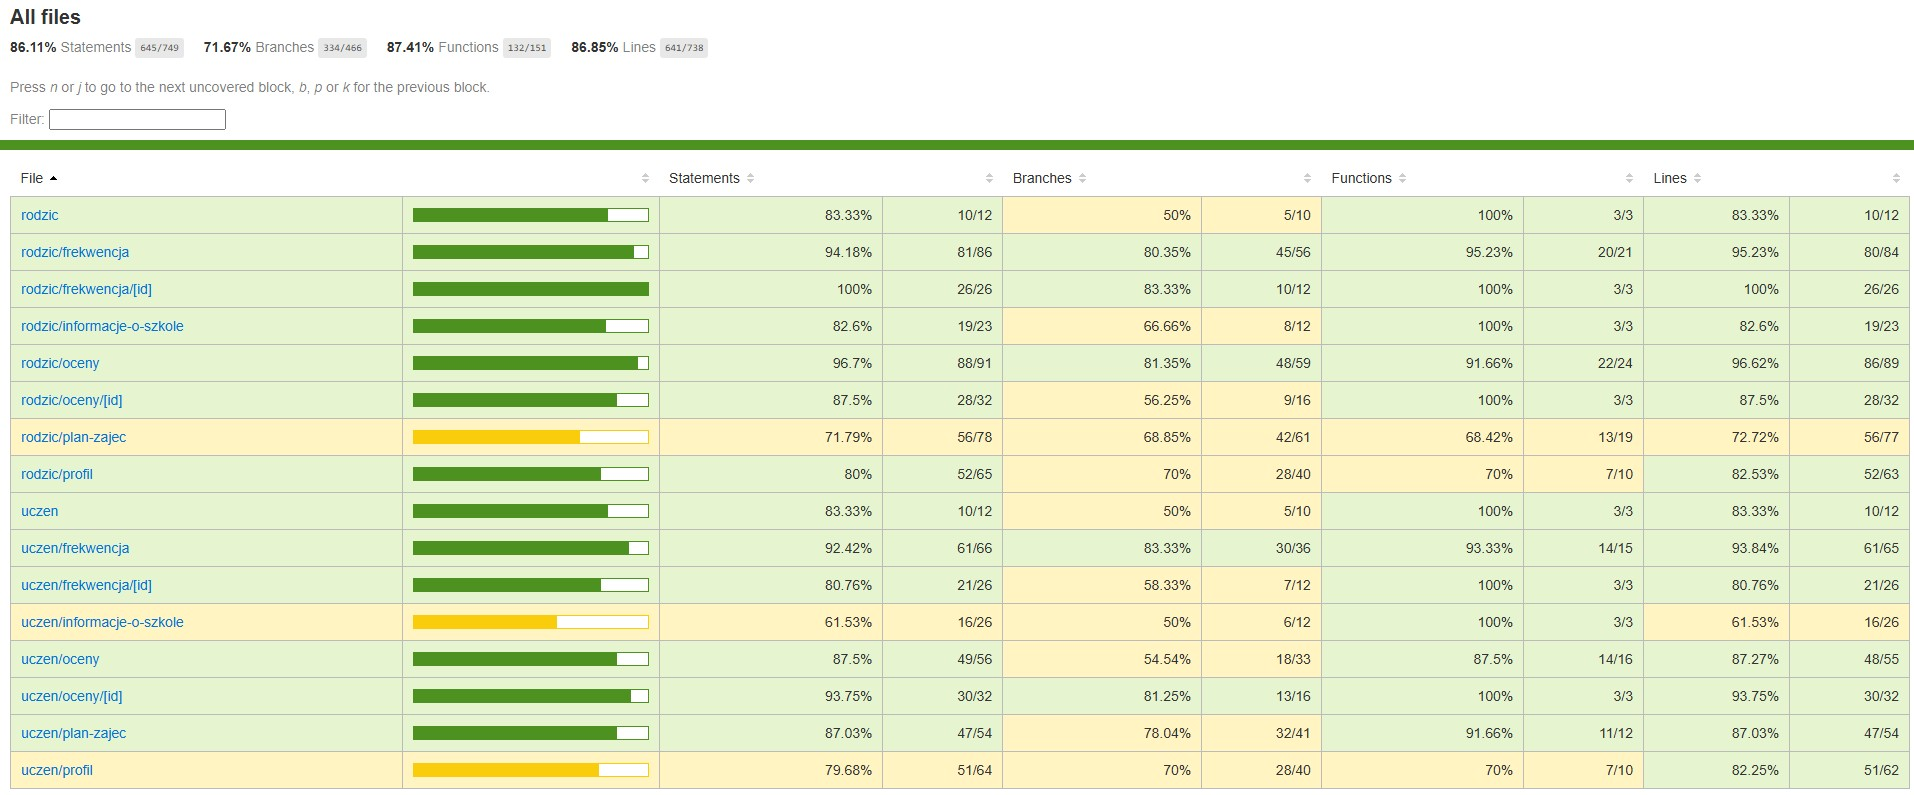
\includegraphics[width=1\textwidth]{obrazy/rozdzial_4/frontend/pokrycie_kodu_uczen_i_rodzic.jpg}
    \caption{Pokrycie kodu dla modułów rodzic i uczen}
\end{figure}

\begin{figure}[H]
    \centering
    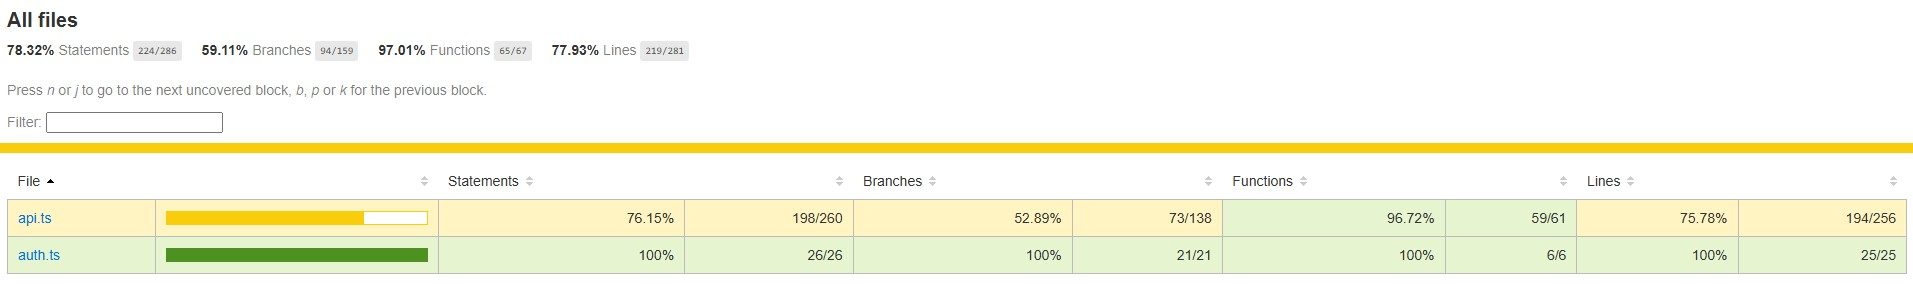
\includegraphics[width=1\textwidth]{obrazy/rozdzial_4/frontend/pokrycie_kodu_lib.jpg}
    \caption{Pokrycie kodu dla modułu lib}
\end{figure}

\begin{figure}[H]
    \centering
    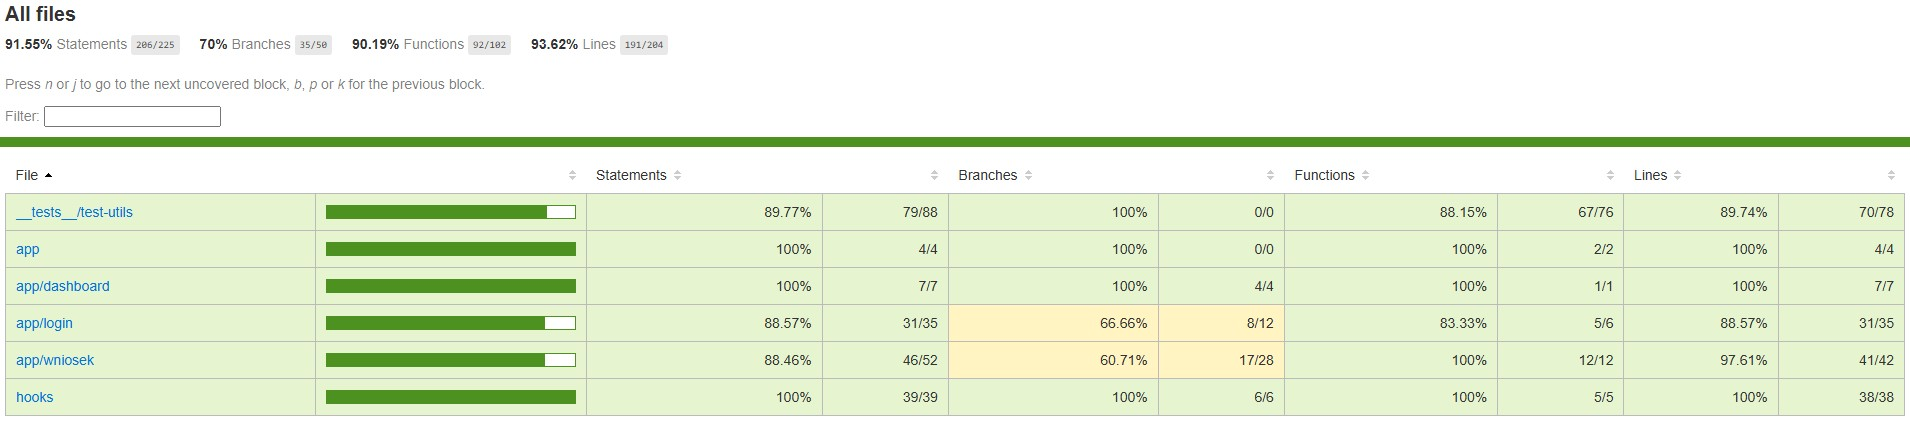
\includegraphics[width=1\textwidth]{obrazy/rozdzial_4/frontend/pokrycie_kodu_pozostale.jpg}
    \caption{Pokrycie kodu dla pozostałych modułów}
\end{figure}

\subsubsection{Kluczowe przypadki testowe}
W procesie tworzenia testów wyznaczono poniższe przypadki testowe:

\paragraph{Testy jednostkowe}
\begin{itemize}
    \item \textbf{Wnioski i szkoły}: Weryfikacja budowania URL, obsługi statusów 201/204 oraz błędnych odpowiedzi (14 przypadków).
    \item \textbf{Operacje CRUD}: Testy operacji dla szkół, użytkowników, klas, uczniów, przedmiotów, lekcji, ocen i frekwencji (14 przypadków).
    \item \textbf{Autoryzacja}: Weryfikacja sesji, przekierowań zależnych od roli oraz uprawnień tras (6 przypadków).
    \item \textbf{Hook useProtectedRoute}: Testy przekierowań przy braku roli, błędach oraz poprawnym dostępie użytkownika (5 przypadków).
\end{itemize}

\paragraph{Testy komponentów}
\begin{itemize}
    \item \textbf{Layout i strony główne}: Renderowanie layoutu aplikacji, strony startowej, dashboardu oraz layoutów ról (9 przypadków).
    \item \textbf{Strony rodzica}: Testy profilu, szkoły, ocen, frekwencji oraz planu zajęć (5 przypadków).
    \item \textbf{Strony ucznia}: Testy profilu, szkoły, ocen, frekwencji oraz planu zajęć (6 przypadków).
    \item \textbf{Widoki szczegółowe}: Testy wyświetlania danych, obsługi błędów pobierania oraz fallbacków identyfikatorów (6 przypadków).
    \item \textbf{Frekwencja i oceny}: Testy błędów, braków danych, zmiany ucznia oraz renderowania warunkowego (11 przypadków).
    \item \textbf{Strony nauczyciela}: Testy frekwencji, ocen i planu zajęć z uwzględnieniem stanów ładowania i błędów (6 przypadków).
    \item \textbf{Administrator szkoły — klasy}: Testy listy klas, tworzenia, usuwania oraz pustego stanu (8 przypadków).
    \item \textbf{Administrator szkoły — szczegóły szkoły}: Testy dodawania administratora, komunikatów, nawigacji oraz renderowania danych (9 przypadków).
    \item \textbf{Administrator szkoły — członkowie}: Testy listy członków, filtrowania, dodawania, usuwania oraz obsługi błędów (11 przypadków).
    \item \textbf{Administrator aplikacji — klasy i użytkownicy}: Testy zarządzania klasami, list uczniów, edycji oraz stanów ładowania (11 przypadków).
    \item \textbf{Administrator aplikacji — wnioski}: Testy listy wniosków, akceptacji, odrzucania oraz podglądu szczegółów (5 przypadków).
    \item \textbf{Logowanie}: Testy procesu logowania, zapisu sesji oraz obsługi błędów (3 przypadki).
    \item \textbf{Przedmioty}: Testy listy przedmiotów, dodawania oraz edycji (5 przypadków).
    \item \textbf{Plan lekcji}: Testy dodawania, usuwania oraz wyświetlania siatki zajęć (4 przypadki).
    \item \textbf{Rozkład godzin}: Testy renderowania godzin oraz dodawania i usuwania wpisów (5 przypadków).
\end{itemize}

\subsubsection{Podsumowanie wyników testów}
\begin{table}[H]
    \centering
    \begin{tabular}{|l|c|c|}
        \hline
        \textbf{Moduł} & \textbf{Liczba testów} & \textbf{Stan} \\ \hline
        Wnioski i szkoły & 14 & 100\% sukces \\ \hline
        Operacje CRUD & 14 & 100\% sukces \\ \hline
        Autoryzacja & 6 & 100\% sukces \\ \hline
        Hook useProtectedRoute & 5 & 100\% sukces \\ \hline
    \end{tabular}
    \caption{Statystyki testów jednostkowych}
\end{table}

\begin{table}[H]
    \centering
    \begin{tabular}{|l|c|c|}
        \hline
        \textbf{Moduł} & \textbf{Liczba testów} & \textbf{Stan} \\ \hline
        Layout i strony główne & 9 & 100\% sukces \\ \hline
        Strony rodzica & 5 & 100\% sukces \\ \hline
        Strony ucznia & 6 & 100\% sukces \\ \hline
        Widoki szczegółowe & 6 & 100\% sukces \\ \hline
        Frekwencja i oceny & 11 & 100\% sukces \\ \hline
        Strony nauczyciela & 6 & 100\% sukces \\ \hline
        Administrator szkoły — klasy & 8 & 100\% sukces \\ \hline
        Administrator szkoły — szczegóły szkoły & 9 & 100\% sukces \\ \hline
        Administrator szkoły — członkowie & 11 & 100\% sukces \\ \hline
        Administrator aplikacji — klasy i użytkownicy & 11 & 100\% sukces \\ \hline
        Administrator aplikacji — wnioski & 5 & 100\% sukces \\ \hline
        Logowanie & 3 & 100\% sukces \\ \hline
        Przedmioty & 5 & 100\% sukces \\ \hline
        Plan lekcji & 4 & 100\% sukces \\ \hline
        Rozkład godzin & 5 & 100\% sukces \\ \hline
    \end{tabular}
    \caption{Statystyki testów komponentów}
\end{table}

\subsection{Analiza testów części backendowej aplikacji}
\subsubsection{Zakres testów}
Testy backendu aplikacji obejmowały weryfikację funkcjonalności poprzez:
\begin{itemize}
    \item 128 testów jednostkowych (JUnit + Mockito).
    \item Pokrycie kodu na poziomie ok. 73 \% (według JaCoCo).
\end{itemize}

Do sprawdzenia pokrycia kodu testami użyto narzędzia JaCoCo (Java Code Coverage), które przedstawia szczegółowe informacje o wykonanych liniach kodu, metodach, klasach oraz rozgałęzieniach warunkowych.

\begin{figure}[H]
    \centering
    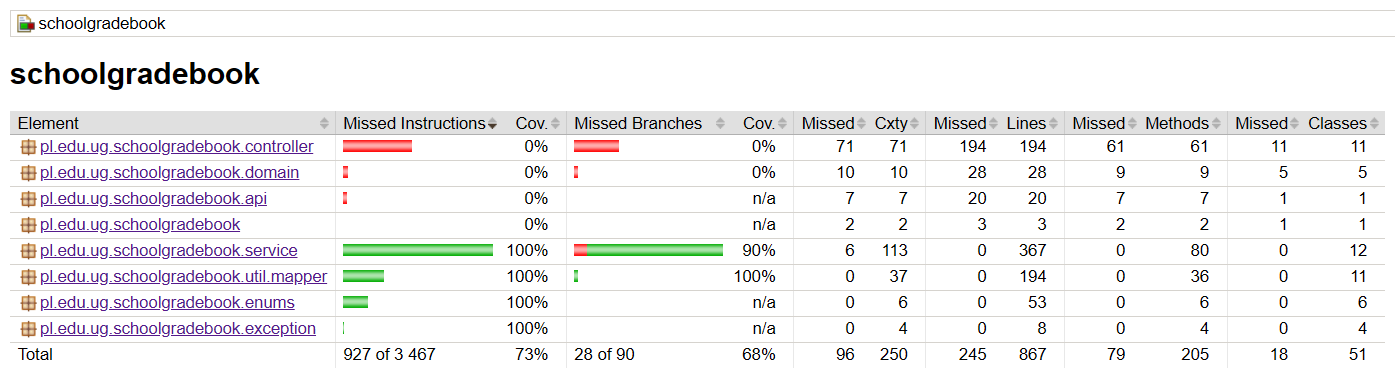
\includegraphics[width=1\textwidth]{obrazy/rozdzial_4/backend/pokrycie_kodu_ogolne.png}
    \caption{Pokrycie kodu dla całej aplikacji backendowej}
\end{figure}

\begin{figure}[H]
    \centering
    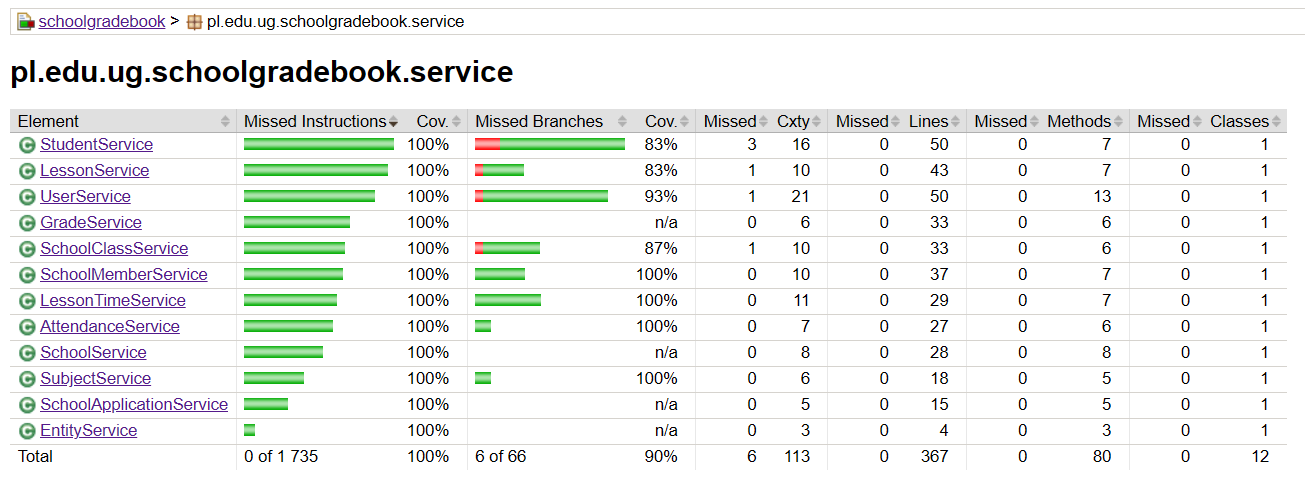
\includegraphics[width=1\textwidth]{obrazy/rozdzial_4/backend/pokrycie_kodu_serwisy.png}
    \caption{Pokrycie kodu dla modułu klas serwisowych}
\end{figure}

\begin{figure}[H]
    \centering
    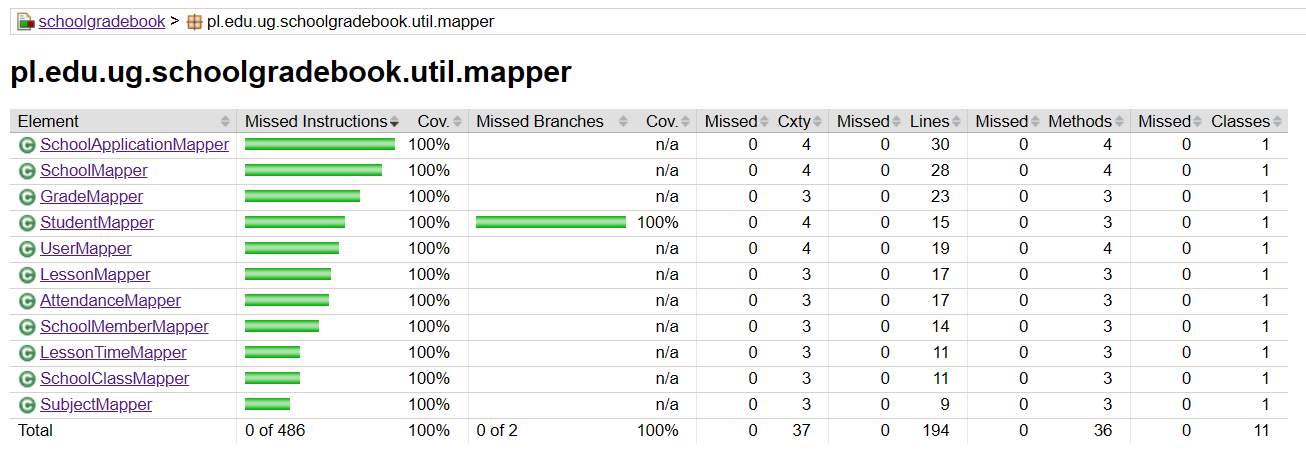
\includegraphics[width=1\textwidth]{obrazy/rozdzial_4/backend/pokrycie_kodu_mappery.png}
    \caption{Pokrycie kodu dla modułu klas mapujących}
\end{figure}

\subsubsection{Kluczowe przypadki testowe}
W procesie tworzenia testów jednostkowych wyznaczono poniższe przypadki testowe:

\begin{itemize}
    \item \textbf{Zarządzanie wnioskami o rejestrację szkoły}: Testy tworzenia, wyszukiwania, edycji i usuwania wniosków (7 przypadków).
    \item \textbf{Zarządzanie szkołami}: Testy tworzenia, wyszukiwania, edycji i usuwania szkół (11 przypadków).
    \item \textbf{Zarządzanie użytkownikami}: Rejestracja, logowanie, edycja, usuwanie, podział na role użytkowników oraz weryfikacja sytuacji kolizyjnych (38 przypadków).
    \item \textbf{Zarządzanie lekcjami}: Tworzenie, wyszukiwanie, edycja, usuwanie lekcji oraz godzin lekcyjnych oraz weryfikacja możliwych kolizji w planach zajęć (18 przypadków).
    \item \textbf{Zarządzanie klasami}: Tworzenie, wyszukiwanie, edycja, usuwanie klas oraz przypisywanie do nich użytkowników (9 przypadków).
    \item \textbf{Zarządzanie przedmiotami szkolnymi}: Tworzenie, wyszukiwanie, edycja, usuwanie przedmiotów i weryfikacja powtórzeń przedmiotów dla szkoły (6 przypadków).
    \item \textbf{Zarządzanie ocenami}: Dodawanie, wyszukiwanie, edycja i usuwanie ocen (6 przypadków).
    \item \textbf{Zarządzanie frekwencją}: Dodawanie, wyszukiwanie, edycja i usuwanie frekwencji (7 przypadków).
    \item \textbf{Mapowanie danych}: Mapowanie obiektów DTO (Data Transfer Object) oraz encji JPA (Java Persistense API) (26 przypadków).
\end{itemize}

\subsubsection{Podsumowanie wyników testów}
\begin{table}[H]
    \centering
    \begin{tabular}{|l|c|c|}
        \hline
        \textbf{Moduł} & \textbf{Liczba testów} & \textbf{Stan} \\ \hline
        Zarządzanie wnioskami & 7 & 100\% sukces \\ \hline
        Zarządzanie szkołami & 11 & 100\% sukces \\ \hline
        Zarządzanie użytkownikami & 38 & 100\% sukces \\ \hline
        Zarządzanie lekcjami & 18 & 100\% sukces \\ \hline
        Zarządzanie klasami & 9 & 100\% sukces \\ \hline
        Zarządzanie przedmiotami & 6 & 100\% sukces \\ \hline
        Zarządzanie ocenami & 6 & 100\% sukces \\ \hline
        Zarządzanie frekwencją & 7 & 100\% sukces \\ \hline
        Mapowanie obiektów & 26 & 100 \% sukces \\ \hline
    \end{tabular}
    \caption{Statystyki testów jednostkowych}
\end{table}

\subsection{Wnioski z testów}
Wszystkie 166 testów po stronie frontendowej zakończyło się powodzeniem, a aplikacja poprawnie obsługuje przypadki brzegowe takie jak brakujące dane, błędy API czy brak uprawnień użytkownika. Dzięki testom jednostkowym kluczowych modułów pomocniczych (api.ts, auth.ts) można było szybko weryfikować poprawność komunikacji z serwerem oraz zarządzania sesją użytkownika. Testy komponentów pozwoliły na weryfikację interakcji między UI, routingiem i logiką biznesową. Osiągnięte pokrycie kodu wynosi 83\% co można uznać za zadowalający wynik.

Wszystkie 128 testów po stronie backendowej zakończyło się powodzeniem, a aplikacja poprawnie zarządza danymi pomiędzy backendem a bazą danych. Testy jednostkowe warstwy serwisowej czy metod mapujących pozwoliły zweryfikować, czy dane są poprawnie mapowane oraz przechowywane w bazie danych. Przetestowano także przypadki konfliktowe pomiędzy danymi np. próba rejestracji na ten sam login czy próba niepoprawnego ustanowienia godzin lekcyjnych. Osiągnięte pokrycie kodu na poziomie 73\% można uznać za dobry wynik.

\end{document}